% Options for packages loaded elsewhere
\PassOptionsToPackage{unicode}{hyperref}
\PassOptionsToPackage{hyphens}{url}
\PassOptionsToPackage{dvipsnames,svgnames*,x11names*}{xcolor}
%
\documentclass[
  11pt,
]{article}
\usepackage{lmodern}
\usepackage{amssymb,amsmath}
\usepackage{ifxetex,ifluatex}
\ifnum 0\ifxetex 1\fi\ifluatex 1\fi=0 % if pdftex
  \usepackage[T1]{fontenc}
  \usepackage[utf8]{inputenc}
  \usepackage{textcomp} % provide euro and other symbols
\else % if luatex or xetex
  \usepackage{unicode-math}
  \defaultfontfeatures{Scale=MatchLowercase}
  \defaultfontfeatures[\rmfamily]{Ligatures=TeX,Scale=1}
\fi
% Use upquote if available, for straight quotes in verbatim environments
\IfFileExists{upquote.sty}{\usepackage{upquote}}{}
\IfFileExists{microtype.sty}{% use microtype if available
  \usepackage[]{microtype}
  \UseMicrotypeSet[protrusion]{basicmath} % disable protrusion for tt fonts
}{}
\makeatletter
\@ifundefined{KOMAClassName}{% if non-KOMA class
  \IfFileExists{parskip.sty}{%
    \usepackage{parskip}
  }{% else
    \setlength{\parindent}{0pt}
    \setlength{\parskip}{6pt plus 2pt minus 1pt}}
}{% if KOMA class
  \KOMAoptions{parskip=half}}
\makeatother
\usepackage{xcolor}
\IfFileExists{xurl.sty}{\usepackage{xurl}}{} % add URL line breaks if available
\IfFileExists{bookmark.sty}{\usepackage{bookmark}}{
\usepackage{hyperref}
}
\hypersetup{
  pdftitle={Cours sur les réseaux informatiques},
  pdfauthor={Première NSI, Lycée du Parc},
  colorlinks=true,
  linkcolor=Maroon,
  filecolor=Maroon,
  citecolor=Blue,
  urlcolor=Blue,
  pdfcreator={LaTeX via pandoc}}
\urlstyle{same} % disable monospaced font for URLs
\usepackage[top=20mm,left=20mm,right=20mm,heightrounded]{geometry}
\usepackage{listings}
\newcommand{\passthrough}[1]{#1}
\lstset{defaultdialect=[5.3]Lua}
\lstset{defaultdialect=[x86masm]Assembler}
\usepackage{longtable,booktabs}
% Correct order of tables after \paragraph or \subparagraph
\usepackage{etoolbox}
\makeatletter
\patchcmd\longtable{\par}{\if@noskipsec\mbox{}\fi\par}{}{}
\makeatother
% Allow footnotes in longtable head/foot
\IfFileExists{footnotehyper.sty}{\usepackage{footnotehyper}}{\usepackage{footnote}}
\makesavenoteenv{longtable}
\usepackage{graphicx}
\makeatletter
\def\maxwidth{\ifdim\Gin@nat@width>\linewidth\linewidth\else\Gin@nat@width\fi}
\def\maxheight{\ifdim\Gin@nat@height>\textheight\textheight\else\Gin@nat@height\fi}
\makeatother
% Scale images if necessary, so that they will not overflow the page
% margins by default, and it is still possible to overwrite the defaults
% using explicit options in \includegraphics[width, height, ...]{}
\setkeys{Gin}{width=\maxwidth,height=\maxheight,keepaspectratio}
% Set default figure placement to htbp
\makeatletter
\def\fps@figure{htbp}
\makeatother
\setlength{\emergencystretch}{3em} % prevent overfull lines
\providecommand{\tightlist}{%
  \setlength{\itemsep}{0pt}\setlength{\parskip}{0pt}}
\setcounter{secnumdepth}{5}

\title{Cours sur les réseaux informatiques}
\usepackage{etoolbox}
\makeatletter
\providecommand{\subtitle}[1]{% add subtitle to \maketitle
  \apptocmd{\@title}{\par {\large #1 \par}}{}{}
}
\makeatother
\subtitle{Thème architectures matérielles et systèmes d'exploitation}
\author{Première NSI, \href{https://frederic-junier.org/}{Lycée du
Parc}}
\date{}

%%%jolis boites

\usepackage{fancybox, graphicx}



%%%%%%%%%%%%%%%%Packages et Macros Frederic%%%%%%%%%%%%%%%%%%%%%%%%%%%%%


%%%%Insertion de liens hypertextes %%%%

            
%%%%%%%%%%PSTricks%%%%%%%%%%%%

\usepackage{pstricks,pst-plot,pst-text,pst-tree,pst-eps,pst-fill,pst-node,pst-math,pstricks-add,pst-xkey,pst-eucl}


%%%%%%%Tikz%%%%%%%%%%%%%%%
\usepackage{pgf,tikz,tkz-tab}
% Pour les tableaux de signes ou de variations avec tkz-tab voir https://zestedesavoir.com/tutoriels/439/des-tableaux-de-variations-et-de-signes-avec-latex/#1-13389_tikz-un-package-qui-en-a-dans-le-ventre
\usetikzlibrary{arrows}
\usetikzlibrary{shapes.geometric}
\usetikzlibrary{shapes.geometric}
\usetikzlibrary{petri}
\usetikzlibrary{decorations}
\usetikzlibrary{arrows}
\usetikzlibrary{math}
 %Variables must be declared in a tikzmath environment but
       % can be used outside
%       \tikzmath{int \n; \n = 508; \x1 = 1; \y1 =1; 
%                   %computations are also possible
%                    \x2 = \x1 + 1; \y2 =\y1 +3; } 


%%%%%%%%%%%%%%%%%%%%%%%%%%%%%%%%%%%%%%%%
%%%%%%%%%%%Commandes Tikz Perso%%%%%%%%%%%%%%%

% Définition des nouvelles options xmin, xmax, ymin, ymax
% Valeurs par défaut : -3, 3, -3, 3
\tikzset{
xmin/.store in=\xmin, xmin/.default=-3, xmin=-3,
xmax/.store in=\xmax, xmax/.default=3, xmax=3,
ymin/.store in=\ymin, ymin/.default=-3, ymin=-3,
ymax/.store in=\ymax, ymax/.default=3, ymax=3,
}
% Commande qui trace la grille entre (xmin,ymin) et (xmax,ymax)
\newcommand {\grille}[2]
{\draw[help lines,black, thick] (\xmin,\ymin) grid[xstep=#1, ystep=#2] (\xmax,\ymax);}
% Commande \axes
\newcommand {\axes} {
\draw[->,very thick] (\xmin,0) -- (\xmax,0);
\draw[->,very thick] (0,\ymin) -- (0,\ymax);
\draw (0.95*\xmax, 0) node[above] {};
\draw (0, 0.95*\ymax) node[left] {};
}
% Commande qui limite l?affichage à (xmin,ymin) et (xmax,ymax)
\newcommand {\fenetre}
{\clip (\xmin,\ymin) rectangle (\xmax,\ymax);}

%Exemple d'utilisation

%\begin{center}
%\begin{tikzpicture} [xmin=-2,xmax=2,ymin=0,ymax=5]
%\grille{1} \axes \fenetre
%\draw plot[smooth] (\x,\x^2);
%\end{tikzpicture}
%\end{center}

%style pour la perspective cavalière française
%voir Tikz pour l'impatient page 68
\tikzset{math3d/.style=
{x= {(-0.353cm,-0.353cm)}, z={(0cm,1cm)},y={(1cm,0cm)}}}

%%%%%%%Symbole pour code calculatrice%%%%%%

%Flèche remplie pour défilement de menu

\newcommand{\flechefillright}{

\begin{tikzpicture}[scale=0.15] \fill (0,0)--(2,1)--(0,2)--cycle;
\end{tikzpicture}}

%%%%%%%%%%%%%Symboles pour calculatrice Casio%%%%
\newcommand{\execasio}{\Pisymbol{psy}{191}} %Retour chariot
\newcommand{\dispcasio}{\begin{pspicture}(.1,.1)\pspolygon*(.1,0)(.1,.1)\end{pspicture}} %Triangle « Disp »
\newcommand{\dispcasiotikz}{
\begin{tikzpicture}[scale=0.2]
\fill (0,0) -- (1,0) -- (1,1) -- cycle;
\end{tikzpicture}} %Triangle « Disp »
%

%Fleche entre deux lignes, d'apres 'un bon petit' : http://forum.mathematex.net/latex-f6/fleches-entre-deux-lignes-pour-resolution-d-equation-t10283.html#p99817
\newcommand\addnode[1]{\Rnode{#1}{}}
\newcommand\linknode[3]{\ncbar[angleA=0,angleB=0,nodesep=1ex,arm=10ex,offset=-2pt]{->}{#1}{#2}\Aput{\vphantom{x}#3}}


%%Commande pour touche de calculatrice

\newcommand\tc[1]{%
{
\begin{tikzpicture}
\node[draw,rectangle,rounded corners=3pt] (P) at (0,0){#1};
\end{tikzpicture}
}
}

%%%%%%%%%%%%%%%%%%%%%%%%%%%%%%%%%%%%%%%%
%%%%%%%%%%%Fin Commandes Tikz%%%%%%%%%%%%%%%


%%%%%%%%%%%%Specifiques%%%%%%%%%%%
\usepackage{wrapfig}
%pour insérer une figure à droite ou à gauche d'un texte
%\begin{wrapfigure}[nb lignes]{placement l,r,c,i(inside),o(outside)}[overhang]{width}
%ce package fonctionne mal à proximité des listes
%%%%%%%%%%%%%%%%%%%%%%%%%%%%%%%%%%%%%

%%%%%Environnements et symboles spéciaux pour faire joli%%%%%%

%%%Bclogo, pour des environnements + jolis avec insertion de logo%%%%
%Dépendances de  bclogo
\usepackage{xkeyval}  
\usepackage{etoolbox}
\usepackage{ifpdf}
\usepackage[framemethod=tikz]{mdframed}
\usepackage[tikz]{bclogo}

%\newcommand\bcpython{
\includegraphics[width=17pt]{/home/fjunier/Maths/python-logo.eps}}
\newcommand\bcpython{
\includegraphics[width=17pt]{/home/fjunier/Maths/python-logo.png}}
%\newcommand\bcpython{
\includegraphics[width=17pt]{/home/frederic/Maths/python-logo.png}}

%% Framed
\usepackage{framed}  %Le package « framed» Crée 3 nouveaux environnements, qui se comportent comme des minipage de largeur \linewidth, mais permettant en plus de se casser entre plusieurs pages.     * framed : avec un cadre autour;     * shaded : avec un fonc coloré (il faut définir la couleur shadecolor);     * leftbar : avec une barre le long du côté gauche.

%%%%%%%%%%%%%%%%%%%Présentation de codes sources%%%%%%%%%%%%%%%%%
\usepackage{listings}
%On utilise l?environnement lstlisting pour insérer
%un code source.
%En plus de l?environnement lstlisting, on peut également utiliser la
%commande \lstinline qui fonctionne comme la commande \verb, en ce
%sens qu?on peut utiliser n?importe quel caractère comme délimiteur. Enfin,
%la commande \lstinputlisting permet de charger un code source depuis
%un fichier externe.
%Il y a deux manières de préciser des options : soit via l?option de l?envi-
%ronnement ou de la commande, soit en utilisant la commande \lstset
%qui permet de définir des options de manière globale.

\lstset{ %
  language=Python,                % the language of the code
  basicstyle=\ttfamily,           % the size of the fonts that are used for the code
  %numbers=left,                   % where to put the line-numbers
  numberstyle=\tiny,  % the style that is used for the line-numbers
  %stepnumber=2,                   % the step between two line-numbers. If it's 1, each line 
                                  % will be numbered
  %numbersep=5pt,                  % how far the line-numbers are from the code
  backgroundcolor=\color{white},      % choose the background color. You must add \usepackage{color}
  showspaces=false,               % show spaces adding particular underscores
  showstringspaces=false,         % underline spaces within strings
  showtabs=false,                 % show tabs within strings adding particular underscores
  frame=single,                   % adds a frame around the code
  rulecolor=\color{black},        % if not set, the frame-color may be changed on line-breaks within not-black text (e.g. comments (green here))
  tabsize=4,                      % sets default tabsize to 2 spaces
  captionpos=b,                   % sets the caption-position to bottom
  breaklines=true,                % sets automatic line breaking
  breakatwhitespace=false,        % sets if automatic breaks should only happen at whitespace
  %title=\lstname,                   % show the filename of files included with \lstinputlisting;
                                  % also try caption instead of title
  breakindent=1cm,
  keywordstyle=\color{blue},          % keyword style
  commentstyle=\color{red},       % comment style
  %stringstyle=\ttfamily\color{green},         % string literal style
  escapeinside={\%*}{*)},            % if you want to add LaTeX within your code
  morekeywords={*,...},              % if you want to add more keywords to the set
  deletekeywords={...}              % if you want to delete keywords from the given language
  upquote=true,columns=flexible,
xleftmargin=1cm,xrightmargin=1cm,
 inputencoding=utf8,			%Les lignes qui suivent sont pour le codage utf8
  extendedchars=true,
  literate=%
            {é}{{\'{e}}}1
            {è}{{\`{e}}}1
            {ê}{{\^{e}}}1
            {ë}{{\¨{e}}}1
            {û}{{\^{u}}}1
            {ù}{{\`{u}}}1
            {â}{{\^{a}}}1
            {à}{{\`{a} }}1
            {î}{{\^{i}}}1
            {ô}{{\^{o}}}1
            {ç}{{\c{c}}}1
            {Ç}{{\c{C}}}1
            {É}{{\'{E}}}1
            {Ê}{{\^{E}}}1
            {À}{{\`{A}}}1
            {Â}{{\^{A}}}1
            {Î}{{\^{I}}}1
}

\lstdefinestyle{rond}{
  numbers=none,
  backgroundcolor=\color{gristclair},
  frameround =tttt
}

\lstdefinestyle{compil}{
  numbers=none,
  backgroundcolor=\color{gristclair}
}
%\lstset{language=Python,basicstyle=\small , frame=single,tabsize=4,showspaces=false,showtabs=false,showstringspaces=false,numbers=left,numberstyle=\tiny , extendedchars=true}



%%%%%%%%%%%%%%%%%%%%%%%%%%%%%%%%%%%%%%%%%%%%%%%%%%%%%%%%%%%%%%%%%%%%%%%%
%%%%%%%%%%%%%%%%%%%%Environnements persos%%%%%%%%%%%%%%%%%%%%%%%%%%%%%%%%
%Syntaxe :
%\newenvironment{nom}[nombre d'args][defaut]{definitions initiales}{definitions finales}
%definitions intiales sont les commandes appelées par \begin{nom}
%Definitions finales sont les commandes appelées par \end{nom}

%%%%%%%%%%%%%%%%Définitions des environnemts persostheoreme, exemple ..%%%%
%%%% Exercice avec encadré %%%%
\newcounter{exo}
\newenvironment{exercice}[1]
{\par \medskip   \addtocounter{exo}{1} \noindent  
\begin{bclogo}[arrondi =0.1,   noborder = true, logo=\bccrayon, marge=4]{~\textbf{Exercice} \textbf{\theexo} {\itshape #1} }  \par}
{
\end{bclogo}
 \par \bigskip }

%%Axiomes, Theoremes, Propriété, Définition, Methode, Preuve


\newenvironment{axiome}[1]
{\par \medskip   \begin{leftbar} \noindent \underline{\textbf{Axiome}}\hspace{0.5cm}{\itshape #1}   \vspace*{10pt} \par }
{\end{leftbar}  \par \medskip }


\newcounter{thme}
\newenvironment{theoreme}[1]
{\par \medskip  \addtocounter{thme}{1} \noindent  
\begin{bclogo}[arrondi =0.1,  ombre = true, barre=none, logo=\bcbook, marge=4]{~\textbf{Théorème} \textbf{\thethme} {\itshape #1} }   \par}
{
\end{bclogo}
 \par \bigskip}

 \newenvironment{theoremedef}[1]
{\par \medskip   \addtocounter{thme}{1} \noindent  
\begin{bclogo}[arrondi =0.1,  ombre = true, barre=none, logo=\bcbook, marge=4]{~\textbf{Théorème-Définition} \textbf{\thethme} {\itshape #1} }   \par}
{
\end{bclogo}
 \par \bigskip }
 
\newcounter{prop}
\newenvironment{propriete}[1]
{\par \medskip   \addtocounter{prop}{1} \noindent  
\begin{bclogo}[arrondi =0.1,  ombre = true, barre=none, logo=\bcbook, marge=4]{~\textbf{Propriété} \textbf{\theprop} {\itshape #1} }   \par}
{
\end{bclogo}
 \par \bigskip }


\newenvironment{corollaire}[1]
{\par \medskip   \noindent  
\begin{bclogo}[arrondi =0.1,  ombre = true, barre=none, logo=\bcbook, marge=4]{~\textbf{Corollaire} {\itshape #1} } \par }
{
\end{bclogo}
 \par \bigskip }

\newenvironment{demo}[1]
{\par \medskip   \noindent  
\begin{bclogo}[arrondi =0.1,  ombre = true, barre=zigzag, noborder = true, logo=\bcloupe, marge=0]{~\textbf{Démonstration} {\itshape #1} } \par \vspace{10pt}}
{
\end{bclogo}
 \par \bigskip }

\newcounter{activite}
\newenvironment{activite}[1]
{\par \medskip   \noindent   \addtocounter{activite}{1}
\begin{bclogo}[arrondi =0.1,   noborder = true, logo=\bcvelo, marge=4]{~\textbf{Activité} \textbf{\theactivite} {\itshape #1} }  \par}
{
\end{bclogo}
 \par \bigskip }


\newenvironment{synthese}
{\par \medskip   \noindent   
\begin{bclogo}[arrondi =0.1,   noborder = true, logo=\bccle, marge=4]{~\textbf{Synthèse}   }  \par}
{
\end{bclogo}
 \par \bigskip }
 
 
\newcounter{rque}
\newenvironment{remarque}
{\par \medskip    \addtocounter{rque}{1} \noindent  
\begin{bclogo}[arrondi =0.1,  ombre = true, barre=snake, noborder = true, logo=\bcinfo, marge=0]{~\textbf{Remarque} \textbf{\therque}}  \par }
{
\end{bclogo}
 \par \bigskip }

\newcounter{def}
\newenvironment{definition}[1]
{\par \medskip   \addtocounter{def}{1} \noindent  
\begin{bclogo}[arrondi =0.1,  ombre = true, barre=none, logo=\bcbook, marge=4]{~\textbf{Définition} \textbf{\thedef} {\itshape #1} }  \par}
{
\end{bclogo}
 \par \bigskip }
 
 
 \newcounter{cours}
\newenvironment{cours}[1]
{\par \medskip   \addtocounter{cours}{1} \noindent  
\begin{bclogo}[arrondi =0.1,  ombre = true, barre=none, logo=\bcbook, marge=4]{~\textbf{Point de cours} \textbf{\thecours} {\itshape #1} }  \par}
{
\end{bclogo}
 \par \bigskip }
 
 

\newenvironment{introduction}
{\par \medskip    \noindent  
 \begin {bclogo}[couleur = blue!5 , arrondi =0.1,logo=\bcrosevents, marge=4] {~\textbf{Introduction}    }
 \par }
{
\end{bclogo}
 \par \bigskip }
 
\newenvironment{memo}[1]
{\par \medskip    \noindent  
\begin{bclogo}[arrondi =0.1,  ombre = true, barre=none, logo=\bccle, marge=4]{~\textbf{À retenir}  {\itshape #1} }  \par}
{
\end{bclogo}
 \par \bigskip }
 
\newcounter{exple}
\newenvironment{exemple}[1]
{\par \medskip   \addtocounter{exple}{1} \noindent  
\begin{bclogo}[arrondi =0.1,   noborder = true, logo=\bclampe, marge=4]{~\textbf{Exemple} \textbf{\theexple} {\itshape #1} }  \par}
{
\end{bclogo}
 \par \bigskip }




\newcounter{alg}
\newenvironment{algorithme}[1]
{\par \medskip   \addtocounter{alg}{1} \noindent  
 \begin {bclogo}[noborder = true, barre=zigzag,logo=\bcpython, marge=4] {~\textbf{Algorithmique} \textbf{\thealg} {\itshape #1} }  \par}
{
\end{bclogo}
 \par \bigskip }

\newcounter{prog}
\newenvironment{programme}[1]
{\par \medskip   \addtocounter{prog}{1} \noindent  
 \begin {bclogo}[noborder = true, barre=zigzag,logo=\bcpython, marge=4] {~\textbf{Programme} \textbf{\theprog} {\itshape #1} }  \par  \bigskip}
{
\end{bclogo}
 \par \bigskip }
 
\newcounter{logi}
\newenvironment{logique}[1]
{\par \medskip   \addtocounter{logi}{1} \noindent  
 \begin {bclogo}[noborder = true, barre=zigzag,logo=\bclampe, marge=4] {~\textbf{Logique} \textbf{\thelogi} {\itshape #1} }  \par}
{
\end{bclogo}
 \par \bigskip }


\newenvironment{methode}[1]
{\par \medskip    \noindent  
 \begin {bclogo}[arrondi =0.1,logo=\bcoutil, marge=4,noborder = true] {~\textbf{Méthode}   {\itshape #1} }  \par}
{
\end{bclogo}
 \par \bigskip }


\newcounter{histo}
\newenvironment{histoire}[1]
{\par \medskip   \addtocounter{histo}{1} \noindent  
 \begin {bclogo}[couleur = blue!10 , arrondi =0.1,logo=\bchorloge, marge=4] {~\textbf{Histoire} \textbf{\thehisto} {\itshape #1} }  \par}
{
\end{bclogo}
 \par \bigskip }




%Environnement contenu pour un document présentant une progression annuelle
\newenvironment{contenu}
{\par \medskip   \begin {bclogo}[ noborder = true,logo=\bccrayon] \noindent {\large \textbf{Contenu de la séance}} \vspace*{10pt} \par  }
{\end{bclogo}  \par \medskip }

%Environnement programme pour un document présentant une progression annuelle
%\newenvironment{programme}
%{\par \medskip   \begin {bclogo}[ noborder = true, barre=zigzag,logo=\bcinfo] \noindent {\large \textbf{Programme officiel}} \vspace*{10pt} \par  }
%{\end{bclogo}  \par \medskip }

%Environnement programme pour un document présentant une progression annuelle
\newenvironment{ressource}
{\par \medskip   \begin {bclogo}[ noborder = true,logo=\bcbook] \noindent {\large \textbf{Ressources}}\\vspace*{10pt} \par }
{\end{bclogo}  \par \medskip }




%%%%%%%%%%%%%%%%%%Maths divers%%%%%%%%%%%%%%%%%%%%%%%%%
%%%%%%%%%%%%%Nombres%%%%%%%%%%%%%%%%

%Ensemble prive de...
%\newcommand{\prive}{\boi}%{\backslash}

%Ensembles de nombres%%%%%%%%%%%%%%%%%
\newcommand{\R}{\mathbb{R}}
\newcommand{\N}{\mathbb{N}}
\newcommand{\D}{\mathbb{D}}
\newcommand{\Z}{\mathbb{Z}}
\newcommand{\Q}{\mathbb{Q}}
%\newcommand{\C}{\mathbb{C}}
\newcommand{\df}{~\ensuremath{]0;+\infty[}~}
\newcommand{\K}{\mathbb{K}}

%%%%%%%%Arithmetique%%%%%%%%%%
%PGCD, PPCM
\newcommand{\PGCD}{\mathop{\rm PGCD}\nolimits}
\newcommand{\PPCM}{\mathop{\rm PPCM}\nolimits}

%Intervalles
\newcommand{\interoo}[2]{]#1\, ;\, #2[}
\newcommand{\Interoo}[2]{\left]#1\, ;\, #2\right[}
\newcommand{\interof}[2]{]#1\, ;\, #2]}
\newcommand{\Interof}[2]{\left]#1\, ;\, #2\right]}
\newcommand{\interfo}[2]{[#1\, ;\, #2[}
\newcommand{\Interfo}[2]{\left[#1\, ;\, #2\right[}
\newcommand{\interff}[2]{[#1\, ;\, #2]}
\newcommand{\Interff}[2]{\left[#1\, ;\, #2\right]}
%\newcommand\interentiers #1#2{[\! [#1\, ;\, #2]\! ]}
\newcommand{\interentiers}[2]{\llbracket #1\, ;\, #2\rrbracket}
%


%%%%%%%%%%%%%%Nombres complexes%%%%%

\newcommand{\ic}{\text{i}}
%\newcommand{\I}{\text{i}}
\newcommand{\im}[1]{\text{Im}\left(#1\right)}
\newcommand{\re}[1]{\text{Re}\left(#1\right)}
\newcommand{\Arg}[1]{\text{arg}\left(#1\right)}
\newcommand{\Mod}[1]{\left[#1\right]}
%Parties entière, réelle, imaginaire, nombre i
\newcommand{\ent}[1]{\text{E}\left(#1\right)}
\renewcommand{\Re}{\mathop{\rm Re}\nolimits}
\renewcommand{\Im}{\mathop{\rm Im}\nolimits}
\renewcommand{\i}{\textrm{i}}

%%%%%%%%%%%Probabilites et statistiques%%%%%
\newcommand{\loibinom}[2]{\mathcal{B}\left(#1\ ; \ #2 \right)}
\newcommand{\loinorm}[2]{\mathcal{N}\left(#1\ ; \ #2 \right)}
\newcommand{\loiexp}[1]{\mathcal{E}\left(#1\right)}
\newcommand{\proba}[1]{\mathbb{P}\big(#1\big)}
\newcommand{\probacond}[2]{\mathbb{P}_{#2}\big(#1\big)}
\newcommand{\esperance}[1]{\mathbb{E}\left(#1\right)}
\newcommand{\variance}[1]{\mathbb{V}\left(#1\right)}
\newcommand{\ecart}[1]{\sigma\left(#1\right)}
\newcommand{\dnormx}{\frac{1}{\sqrt{2\pi}} \text{e}^{-\frac{x^2}{2}}}
\newcommand{\dnormt}{\frac{1}{\sqrt{2\pi}} \text{e}^{-\frac{t^2}{2}}}

%Covariance
\newcommand{\cov}{\mathop{\rm cov}\nolimits}
%


%%%%%%%%%%Analyse%%%%%%%%%%%

%%%%%%%%%%%Courbe%%%%%%%%%%%%
\newcommand{\courbe}[1]{\ensuremath{\mathcal{C}_{#1}}}

%%%%%%%Fonction exponentielle%%%%%
\newcommand{\fe}{~fonction exponentielle~}
\newcommand{\e}{\text{e}}

%Fonction cotangente
\newcommand{\cotan}{\mathop{\rm cotan}\nolimits}
%%%%%%%%%%%%%%%%%%%%%%%%%%%%%%%%%%%%%%%%%
%
%Fonctions hyperboliques
\newcommand{\ch}{\mathop{\rm ch}\nolimits}
\newcommand{\sh}{\mathop{\rm sh}\nolimits}


%%%%%%%%%%%%%%Limites%%%%%%
\newcommand{\limite}[2]{\lim\limits
_{x \to #1} #2}
\newcommand{\limitesuite}[1]{\lim\limits
_{n \to +\infty} #1}
\newcommand{\limiteg}[2]{\lim\limits
_{\substack{x \to #1 \\ x < #1 }} #2}
\newcommand{\limited}[2]{\lim\limits
_{\substack{x \to #1 \\ x > #1 }} #2}

%%%%%%%%%%Continuité%%%%%%%%%%%
\newcommand{\TVI}{théorème des valeurs intermédiaires}

%%%%%%%%%%%Suites%%%%%%%%%%%%
\newcommand{\suite}[1]{\ensuremath{\left(#1_{n}\right)}}
\newcommand{\Suite}[2]{\ensuremath{\left(#1\right)_{#2}}}
%

%%%%%%%%%%%%%%%Calcul intégral%%%%%%
\newcommand{\dx}{\ensuremath{\text{d}x}}		% dx
\newcommand{\dt}{\ensuremath{\text{d}t}}		% dt
\newcommand{\dtheta}{\ensuremath{\text{d}\theta}}		% dtheta
\newcommand{\dy}{\ensuremath{\text{d}y}}		% dy
\newcommand{\dq}{\ensuremath{\text{d}q}}		% dq

%%%Intégrale%%%
\newcommand{\integralex}[3]{\int_{#1}^{#2} #3 \ \dx}
\newcommand{\integralet}[3]{\int_{#1}^{#2} #3 \ \dt}
\newcommand{\integraletheta}[3]{\int_{#1}^{#2} #3 \ \dtheta}

%%%%%Equivalent%%
\newcommand{\equivalent}[1]{\build\sim_{#1}^{}}

%o et O%%%%
\renewcommand{\o}[2]{\build o_{#1\to #2}^{}}
\renewcommand{\O}[2]{\build O_{#1\to #2}^{}}



%%%%%%%%%%%%%%%Geometrie%%%%%%%%%%%%%%%%%%%%%%%

%%%%%%%%%%%%%%%Reperes%%%%%%%%%%%%%%
\def\Oij{\ensuremath{\left(\text{O},~\vect{\imath},~\vect{\jmath}\right)}}
\def\Oijk{\ensuremath{\left(\text{O},~\vect{\imath},~ \vect{\jmath},~ \vect{k}\right)}}
\def\Ouv{\ensuremath{\left(\text{O},~\vect{u},~\vect{v}\right)}}
\renewcommand{\ij}{(\vec\imath\, ;\vec\jmath\,)}
\newcommand{\ijk}{(\vec\imath\, ;\vec\jmath\, ;\vec k\,)}
\newcommand{\OIJ}{(O\,;\, I\,;\, J\,)}
\newcommand{\repere}[3]{\big(#1\, ;\,\vect{#2} ;\vect{#3}\big)}
\newcommand{\reperesp}[4]{\big(#1\, ;\,\vect{#2} ;\vect{#3} ;\vect{#4}\big)}

%%%%%%%%%Coordonnees%%%%%%%%%%%%%%
\newcommand{\coord}[2]{(#1\, ;\, #2)}
\newcommand{\bigcoord}[2]{\big(#1\, ;\, #2\big)}
\newcommand{\Coord}[2]{\left(#1\, ;\, #2\right)}
\newcommand{\coordesp}[3]{(#1\, ;\, #2\, ;\, #3)}
\newcommand{\bigcoordesp}[3]{\big(#1\, ;\, #2\, ;\, #3\big)}
\newcommand{\Coordesp}[3]{\left(#1\, ;\, #2\, ;\, #3\right)}
\newcommand{\Vcoord}[3]{\begin{pmatrix} #1 \\ #2 \\ #3 \end{pmatrix}}
%Symboles entre droites
%\newcommand{\paral}{\sslash}
\newcommand{\paral}{\mathop{/\!\! /}}
%

%%%%%%%%%Produit scalaire, Angles%%%%%%%%%%
\newcommand{\scal}[2]{\vect{#1} \, \cdot \, \vect{#2}}
\newcommand{\Angle}[2]{\left(\vect{#1} \, , \, \vect{#2}\right)}
\newcommand{\Anglegeo}[2]{\left(\widehat{\vect{#1} \, ; \, \vect{#2}}\right)}
\renewcommand{\angle}[1]{\widehat{#1}}
\newcommand{\anglevec}[2]{\left(\vect {#1}\, ,\,\vect {#2} \right)}
\newcommand{\anglevecteur}[2]{(#1\, , \, #2)}
\newcommand{\Anglevec}[2]{(\vecteur{#1}\, ,\,\vecteur{#2})}
\newcommand{\prodscal}[2]{#1 \, \cdot \, #2}
%


%Arc
%\newcommand{\arc}[1]{\wideparen{#1}}
\newcommand{\arcoriente}[1]{\overset{\curvearrowright}{#1}}
%
%


%%%%%%%%%%%%%%%Normes%%%%%%%%%%%%%%%%
\newcommand{\norme}[1]{\left\| #1\right\|}
\newcommand{\normebis}[1]{\delim{2pt}{\|}{9pt}\! #1\delim{2pt}{\|}{9pt}}
\newcommand{\normetriple}[1]{\left |\kern -.07em\left\| #1\right |\kern -.07em\right\|}
\newcommand{\valabs}[1]{\big| \, #1 \, \big|}
%

%%%%%%%%%%%%%%%%%%%%%%%%%%%Degré%%%%%%
%\newcommand{\Degre}{\ensuremath{^\circ}}
%La commande \degre est déjà définie dans le package babel

%%%%%%%%%%Vecteurs%%%%%%%%%%%
\newcommand{\vect}[1]{\mathchoice%
{\overrightarrow{\displaystyle\mathstrut#1\,\,}}%
{\overrightarrow{\textstyle\mathstrut#1\,\,}}%
{\overrightarrow{\scriptstyle\mathstrut#1\,\,}}%
{\overrightarrow{\scriptscriptstyle\mathstrut#1\,\,}}}



%%%%%%%%%%%%%Algebre%%%%%%%%%%%%%%%


%%%%%%%%%%Systemes%%%%%%%%%%%
%Systemes
\newcommand{\sys}[2]{
\left\lbrace
 \begin{array}{l}
  \negthickspace\negthickspace #1\\
  \negthickspace\negthickspace #2\\
 \end{array}
\right.\negthickspace\negthickspace}
\newcommand{\Sys}[3]{
\left\lbrace
 \begin{array}{l}
  #1\\
  #2\\
  #3\\
 \end{array}
\right.}
\newcommand{\Sysq}[4]{
\left\lbrace
 \begin{array}{l}
  #1\\
  #2\\
  #3\\
  #4\\
 \end{array}
\right.}
%
%

%%%%%%%%%%%%%%%%Matrices%%%%%%%%%%%%%%%%%%
%Comatrice
\newcommand{\com}{\mathop{\rm com}\nolimits}
%
%
%Trace
\newcommand{\tr}{\mathop{\rm tr}\nolimits}
%
%
%Transposee
\newcommand{\transposee}[1]{{\vphantom{#1}}^t\negmedspace #1}
%
%
%Noyau
\newcommand{\Ker}{\mathop{\rm Ker}\nolimits}
%
%

%
%Matrices
\newcommand{\Mn}{\mathcal M_n}
\newcommand{\matrice}[4]{
\left(
 \begin{array}{cc}
  #1 & #2 \\
  #3 & #4
 \end{array}
\right)}

\newcommand{\Matrice}[9]{
\left(
 \begin{array}{ccc}
  #1 & #2 & #3\\
  #4 & #5 & #6\\
  #7 & #8 & #9
 \end{array}
\right)}
\newcommand{\Vect}[3]{
\left(\negmedspace
 \begin{array}{c}
  #1\\
  #2\\
  #3
 \end{array}\negmedspace
\right)}
\newcommand{\Ideux}{\matrice{1}{0}{0}{1}}
\newcommand{\Itrois}{\Matrice{1}{0}{0}{0}{1}{0}{0}{0}{1}}
%
%
%Determinants
\newcommand{\determinant}[4]{
\left|
 \begin{array}{cc}
  #1 & #2 \\
  #3 & #4
 \end{array}
\right|}
\newcommand{\Determinant}[9]{
\left|
 \begin{array}{ccc}
  #1 & #2 & #3\\
  #4 & #5 & #6\\
  #7 & #8 & #9
 \end{array}
\right|}

\begin{document}
\maketitle

\renewcommand*\contentsname{Table des matières}
{
\hypersetup{linkcolor=}
\setcounter{tocdepth}{3}
\tableofcontents
}
\hypertarget{cruxe9dits}{%
\section*{Crédits}\label{cruxe9dits}}
\addcontentsline{toc}{section}{Crédits}

\emph{Ce cours est largement inspiré du chapitre 26 au manuel NSI de la
collection Tortue chez Ellipse, auteurs : Ballabonski, Conchon,
Filliatre, N'Guyen. Ce document est aussi constitué de nombreux emprunts
à des ressources en ligne proposées par les collègues du
\href{http://portail.lyc-la-martiniere-diderot.ac-lyon.fr/srv1/co/Div_6_Archi_OS_3.html}{lycée
La Martinière Diderot de Lyon},
\href{http://archives.janviercommelemois.fr/nsi/fichiers_pdf/feuille-internet.pdf}{Romain
Janvier} ou
\href{https://pixees.fr/informatiquelycee/n_site/nsi_prem.html}{David
Roche}.}

\hypertarget{ruxe9seau-informatique}{%
\section{Réseau informatique}\label{ruxe9seau-informatique}}

\hypertarget{histoire}{%
\subsection{Histoire}\label{histoire}}

\begin{histoire}{}

Il existait déjà des réseaux locaux reliant directement des ordinateurs
dans les années \(1950\).

À partir des années \(1960\), des chercheurs ont réfléchi à la
problématique de l'interconnexion de réseaux hétérogènes.

Le principe de la \textbf{transmission de paquets} est introduit par
\href{https://fr.wikipedia.org/wiki/Paul_Baran}{Paul Baran et Davies} en
1961 : il consiste à découper les données en paquets, ce qui permet de
transmettre à débit variable (un courriel nécessite l'envoi ponctuel de
petits paquets alors que pour un transférer un fichier, il faut envoyer
rapidement de gros paquets).

\href{https://interstices.info/une-breve-histoire-des-reseaux-de-telecommunications/}{Arpanet},
le projet de réseau interuniversitaire financé par \emph{l'Arpa} (agence
de recherche de la défense américaine) , voit le jour en 1969 sous la
direction de
\href{https://fr.wikipedia.org/wiki/Leonard_Kleinrock}{Leonard
Kleinrock} : les données sont découpées en paquets transmis en séquence
les uns à la suite des autres.

Dans les années 70,
\href{https://interstices.info/louis-pouzin-la-tete-dans-les-reseaux/}{Louis
Pouzin}, après un séjour au \href{http://www.mit.edu/}{MIT}, développe
en France le réseau \emph{Cyclades} qui est le premier véritable réseau
à \textbf{commutation de paquets}: les paquets transitent de façon
indépendante dans le réseau grâce à un protocole qui préfigure
\href{}{Internet Protcol} puis sont remis en l'ordre à l'arrivée. Le
circuit des paquets est donc variable contrairement à la
\textbf{commutation de circuits} implémentée dans le réseau
téléphonique.

\href{https://interstices.info/une-breve-histoire-des-reseaux-de-telecommunications/}{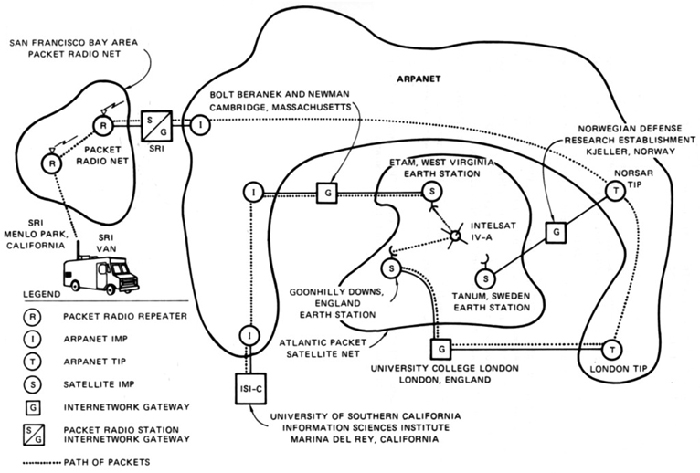
\includegraphics{images/internet-1977.jpg}!}

Aux États-Unis, \href{https://fr.wikipedia.org/wiki/Vint_Cerf}{Vinton
Cerf et Robert Kahn} s'inspirent des idées de Pouzin et inventent les
protocoles \textbf{IP} et \textbf{TCP}. L'interconnexion des réseaux
Arpanet et Csnet en 1983 avec \textbf{TCP/IP} marque la naissance
d'Internet et son expansion au niveau mondial dans les sphères
universitaires et de la recherche.

En 1989,
\href{https://interstices.info/les-debuts-du-web-sous-loeil-du-w3c/}{Tim
Berners-Lee} invente le \textbf{Web}, qui est une application de
documents hypertexte s'exécutant par-dessus le réseau \textbf{Internet}.
L'ouverture des protocoles Web au grand public en 1993 connaît un succès
fulgurant, d'autres services Internet comme le Mail ou le transfert de
fichier de Pair à pair se popularisent aussi et le trafic Internet
explose : de quelques Megabits par secondes en 1992, on est passé à près
de 100 Terabits par seconde en 2018 avec près de 3,2 milliards
d'internautes en 2016.

\end{histoire}

\begin{figure}
\centering
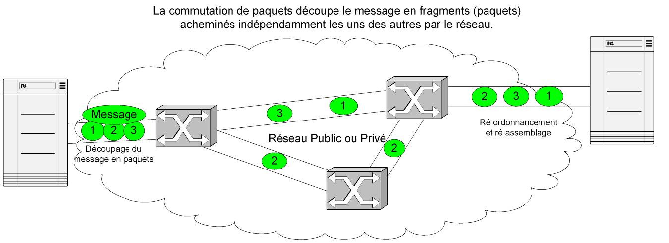
\includegraphics{images/commutationpaquets.png}
\caption{Commutation de paquets}
\end{figure}

\hypertarget{terminologie-et-classification-des-ruxe9seaux}{%
\subsection{Terminologie et classification des
réseaux}\label{terminologie-et-classification-des-ruxe9seaux}}

\begin{definition}{}

\begin{enumerate}
\def\labelenumi{\arabic{enumi}.}
\tightlist
\item
  Un \textbf{réseau} est un ensemble de \emph{noeuds} reliés par des
  \emph{liens}, qui correspond mathématiquement à un \emph{graphe}. Dans
  un \textbf{réseau informatique} les \emph{noeuds} ou \emph{hôtes} sont
  des des équipements informatiques comme des ordinateurs, des routeurs
  \ldots{} et les \emph{liens} peuvent être variées selon la technologie
  utilisée : filaire (Ethernet, \ldots) ou par ondes (Wifi, \ldots).
\item
  Une \textbf{interface} est le point de raccordement, matériel (carte
  réseau) ou logiciel, entre un \emph{lien} et un \emph{noeud}.
\item
  Un \textbf{protocole} est un ensemble de règles permettant d'établir
  une communication entre deux noeuds du réseau et de garantir
  éventuellement certains services (fiabilité, confidentialité \ldots.)
\item
  Un \textbf{service réseau} est une \emph{application} capable de
  communiquer en réseau et proposant des fonctionnalités. Par exemple,
  un service Web peut fournir des pages Web au navigateur d'un client
  les pages Web qu'il demande. Sur un réseau pédagogique de lycée, un
  service de gestion et de partage de fichiers permet aux utilisateurs
  d'accéder à leurs fichiers depuis n'importe quel machine cliente.
\item
  Un \textbf{serveur} désigne un matériel ou un logiciel exécutant un
  \textbf{service réseau}. Il fournit un service à des \textbf{clients}
  selon une \textbf{architecture client / serveur}. Pour une
  présentation de l'architecture client-serveur, on pourra visionner
  cette \href{https://vimeo.com/138623558}{video}.
\end{enumerate}

\end{definition}

\begin{figure}
\centering
\includegraphics[width=0.6\textwidth,height=\textheight]{images/500px-Modèle-client-serveur.svg.png}
\caption{Architecture client / serveur (Wikimedia Commons)}
\end{figure}

\begin{cours}{}

\begin{itemize}
\tightlist
\item
  Les réseaux informatiques peuvent être de différentes tailles :

  \begin{itemize}
  \tightlist
  \item
    Les r\emph{éseaux locaux} ou \textbf{Local Area Network (LAN)}
    limités à une zone géographique restreinte (maison, entreprise,
    lycée \ldots)
  \item
    Les \emph{réseaux étendus} ou \textbf{Wide Area Network (WAN)}
    couvrant de vastes zones géographiques (pays, continent ). Ce sont,
    par exemple, les réseaux des fournisseurs d'accès internet (Free,
    Orange, SFR\ldots), de grandes sociétés\ldots{}
  \item
    Internet est une interconnexion mondiale de réseaux
  \end{itemize}
\item
  Les réseaux informatiques utilisent des liens de technologies diverses
  :

  \begin{itemize}
  \tightlist
  \item
    Des liaisons filaires :

    \begin{itemize}
    \tightlist
    \item
      \emph{câbles à paires torsadées} utilisées avec le protocole de
      liaison Ethernet dans les \textbf{LAN} : sensibles aux
      interférences électromagnétiques même s'ils sont blindés, leur
      portée maximale est de 200 mètres avec un débit maximal de 1 Gb/s
      ;
    \item
      \emph{fibres optiques} utilisées pour les interconnexions de
      réseau (dont les câbles sous-marin pour les liaisons
      intercontinentales) avec un débit de plusieurs Gb/s et des
      contraintes de portée réduites (sauf pour l'hypertrading des
      places financières !)
    \end{itemize}
  \item
    Des liaisons par ondes : Wifi, Bluetooth, Satellite, 4G \ldots{}
  \end{itemize}
\item
  L'interconnexion dans l'Internet de tous ces réseaux hétérogènes sur
  le plan matériel, a été rendu possible par le développement de
  \textbf{protocoles logiciels}. Pour une présentation globale
  d'Internet, on pourra visionner cette
  \href{https://youtu.be/dCknqcjcItU}{video}.
\end{itemize}

\end{cours}

\begin{figure}
\centering
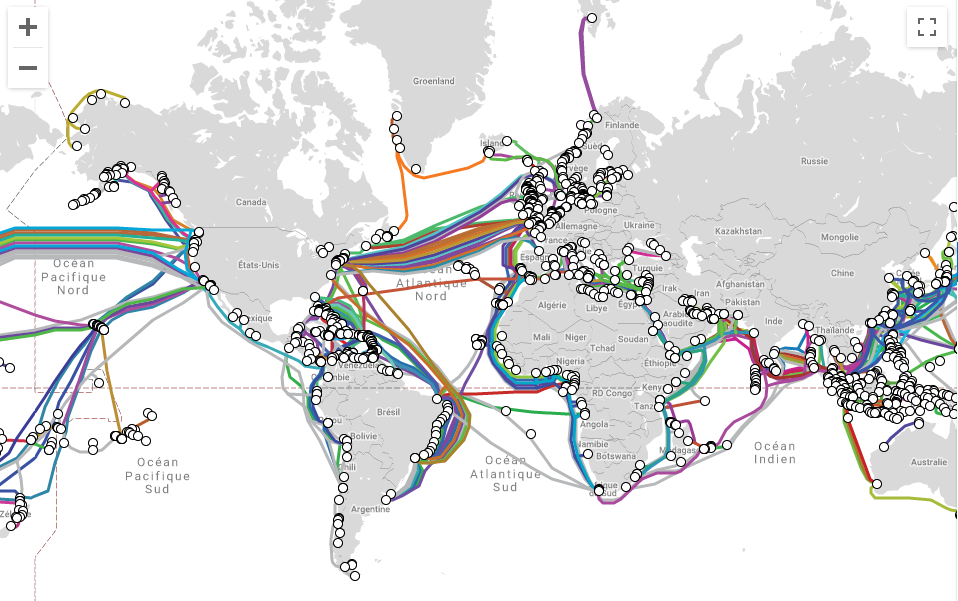
\includegraphics[width=0.7\textwidth,height=\textheight]{images/cable-sousmarin.png}
\caption{Cartes des câbles sous-marins :
\url{https://www.submarinecablemap.com/}}
\end{figure}

\begin{exercice}{}

\emph{QCM type E3C}

\begin{enumerate}
\def\labelenumi{\arabic{enumi}.}
\tightlist
\item
  Un protocole est un ensemble de \ldots{}
\end{enumerate}

\begin{itemize}
\tightlist
\item
  \textbf{Réponse A :} matériels connectés entre eux
\item
  \textbf{Réponse B :} serveurs et de clients connectés entre eux
\item
  \textbf{Réponse C :} règles qui régissent les échanges entre
  équipements informatiques
\item
  \textbf{Réponse D :} règles qui régissent les échanges entre un
  système d'exploitation et les applications
\end{itemize}

\begin{enumerate}
\def\labelenumi{\arabic{enumi}.}
\setcounter{enumi}{1}
\tightlist
\item
  Comment s'appelle l'ensemble des règles qui régissent les échanges sur
  Internet ?
\end{enumerate}

\begin{itemize}
\tightlist
\item
  \textbf{Réponse A :} les couches
\item
  \textbf{Réponse B :} le wifi
\item
  \textbf{Réponse C :} les protocoles
\item
  \textbf{Réponse D :} les commutateurs
\end{itemize}

\begin{enumerate}
\def\labelenumi{\arabic{enumi}.}
\setcounter{enumi}{2}
\tightlist
\item
  L'architecture client-serveur :
\end{enumerate}

\begin{itemize}
\tightlist
\item
  \textbf{Réponse A :} est un mode de communication entre programmes
\item
  \textbf{Réponse B :} est une architecture matérielle de coopération
  entre machines
\item
  \textbf{Réponse C :} est un mode de communication entre routeurs
\item
  \textbf{Réponse D :} est un mode de communication entre commutateurs
\end{itemize}

\end{exercice}

\hypertarget{le-moduxe8le-en-couches}{%
\section{Le modèle en couches}\label{le-moduxe8le-en-couches}}

\hypertarget{duxe9coupage-des-donnuxe9es-en-paquets}{%
\subsection{Découpage des données en
paquets}\label{duxe9coupage-des-donnuxe9es-en-paquets}}

\begin{cours}{}

Dans un réseau informatique, si on veut transmettre une image de
plusieurs Méga octets, on n'envoie pas les données en un seul bloc mais
on les découpe en paquets plus petits qui sont transmis séparément.
Ainsi, il n'est pas nécessaire de tout retransmettre en cas d'erreur de
plus cela réduit les risques d'encombrement o ude blocage des liens.

Ce principe de \textbf{découpage des données en paquets} s'appelle le
\textbf{multiplexage}

\end{cours}

\includegraphics[width=0.6\textwidth,height=\textheight]{images/multiplex2.gif}\\

\emph{Réseau sans multiplexage : canal bloqué}

\includegraphics[width=0.6\textwidth,height=\textheight]{images/multiplex4.gif}\\

\emph{Réseau avec multiplexage}

\hypertarget{moduxe8le-en-couches-et-encapsulation-des-donnuxe9es}{%
\subsection{Modèle en couches et encapsulation des
données}\label{moduxe8le-en-couches-et-encapsulation-des-donnuxe9es}}

\begin{cours}{}

L'interconnexion de réseaux hétérogènes et éloignés géographiquement
nécessite de gérer des problématiques à plusieurs niveaux :

\begin{enumerate}
\def\labelenumi{\arabic{enumi}.}
\tightlist
\item
  la liaison physique entre deux \emph{noeuds} / \emph{hôtes} du réseau
  ;
\item
  l'interconnexion entre deux réseaux locaux ;
\item
  la transmission fiable des données ;
\item
  la communication entre une application s'exécutant sur un client et un
  service réseau sur un serveur.
\end{enumerate}

Les recherches et les expériences menées dans les années 60/70 sur les
réseaux informatiques ont conduit au développement de solutions basées
sur une \textbf{architecture en pile de protocoles logiciels}. Les
problèmes ont été séparés en \textbf{couches}. Le
\href{https://fr.wikipedia.org/wiki/Mod\%C3\%A8le_OSI}{modèle OSI}
comporte sept couches, c'est un modèle théorique et normalisé qui permet
d'encadrer la création de nouveaux protocoles. En pratique, Internet
s'appuie sur le
\href{https://fr.wikipedia.org/wiki/Suite_des_protocoles_Internet}{modèle
TCP/IP} en quatre couches correspondant aux quatre niveaux de problèmes
précités. De la couche la plus basse à la plus haute on distingue :

\begin{enumerate}
\def\labelenumi{\arabic{enumi}.}
\tightlist
\item
  la \emph{couche liaison}
\item
  la \emph{couche réseau}
\item
  la \emph{couche transport}
\item
  la \emph{couche application}
\end{enumerate}

Lorsqu'un hôte A du réseau communique avec un hôte B, chaque couche de
protocole sur l'émetteur communique avec la couche de même niveau chez
le destinataire.

Chaque couche ajoute des \emph{metadonnées} aux données du message qui
sont encapsulées les unes dans les autres. C'est le principe
d'\textbf{encapsulation des données}.

Lors de l'émission le message par l'hôte A, les couches s'exécutent de
haut en bas pour l'encapsulation :

\begin{itemize}
\tightlist
\item
  un protocole de la \emph{couche application} encapsule le message avec
  un entête contenant ses \emph{metadonnées} et transmet
  \emph{application(message)} à la couche inférieure
\item
  puis une protocole de la \emph{couche transport} ajoute son entête :
  \emph{transport(application(message))}
\item
  puis un protocole de la \emph{couche réseau} fait de même :
  \emph{réseau(transport(application(message)))}
\item
  et enfin un protocole de la \emph{couche liaison} transmet le message
  sur le support avec un dernier entête :
  \emph{liaison(réseau(transport(application(message))))}
\end{itemize}

À réception du message par l'hôte B, les couches d'exécutent en ordre
inverse pour désencapsuler le message :

\begin{itemize}
\tightlist
\item
  un protocole de la \emph{couche liaison} extrait et analyse l'entête
  \emph{liaison} ajouté par son homologue et transmet
  \emph{réseau(transport(application(message)))} à la couche supérieure
\item
  un protocole de la \emph{couche réseau} extrait et analyse l'entête
  \emph{réseau} ajouté par son homologue et transmet
  \emph{transport(application(message))} à la couche supérieure
\item
  de même un protocole de la couche \emph{transport} extrait un entête
  et transmet \emph{application(message)} à la couche supérieure
  \emph{application}
\item
  un protocole de la couche \emph{application} extrait le dernier entête
  et transmet le \emph{message} à l'application destinataire.
\end{itemize}

Dans ces deux phases, on voit qu'un protocole doit pouvoir communiquer
avec un protocole de couche immédiatement inférieure ou supérieure par
le biais d'une \textbf{interface}.

\textbf{L'encapsulation des données} permet d'isoler les fonctionnalités
et de développer indépendamment les protocoles de différentes couches.

\end{cours}

\begin{figure}
\centering
\includegraphics{images/osi_couches.gif}
\caption{Encapsulation des données}
\end{figure}

\begin{figure}
\centering
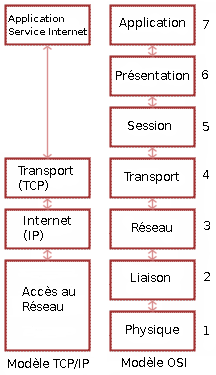
\includegraphics{images/pileTCPIP2.png}
\caption{Modèles en couches : OSI et TCP/IP}
\end{figure}

\begin{exercice}{}

\emph{QCM type E3C}

Quel est le principe de l'encapsulation des données dans un réseau
informatique ?

\begin{itemize}
\tightlist
\item
  \textbf{Réponse A :} Cacher les données afin que l'on ne puisse pas
  les lire
\item
  \textbf{Réponse B :} Mettre les données les unes à la suite des autres
\item
  \textbf{Réponse C :} Inclure les données d'un protocole dans un autre
  protocole
\item
  \textbf{Réponse D :} Chiffrer les données afin que l'on ne puisse pas
  les lire
\end{itemize}

\end{exercice}

\hypertarget{la-couche-liaison-du-moduxe8le-tcpip}{%
\subsection{La couche liaison du modèle
TCP/IP}\label{la-couche-liaison-du-moduxe8le-tcpip}}

\begin{figure}
\centering
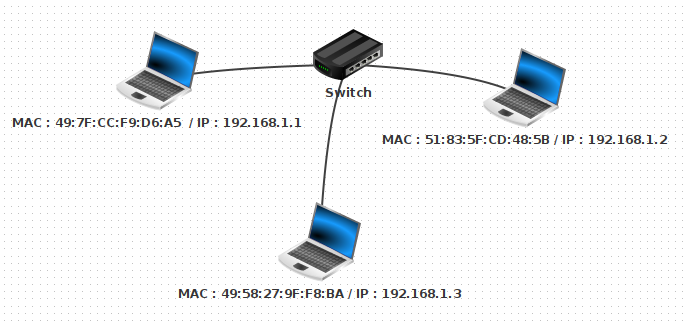
\includegraphics{images/lan2.png}
\caption{Un réseau local Ethernet avec 3 hôtes et un switch}
\end{figure}

\begin{activite}{}

\begin{enumerate}
\def\labelenumi{\arabic{enumi}.}
\item
  Ouvrir avec le logiciel
  \href{https://www.lernsoftware-filius.de/Herunterladen}{Filius} le
  fichier \passthrough{\lstinline!lan2.fls!}. Quels sont les équipements
  présents dans ce réseau ? Sélectionner le mode \emph{construction}
  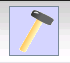
\includegraphics[width=0.1\textwidth,height=\textheight]{images/filius-construction.png}~Faire
  un clic droit sur chacune des machines du réseau, sélectionner
  \emph{Configurer} et noter leur adresse MAC. Il s'agit d'un
  identifiant pour chaque matériel constitué de 6 paquets de 8 bits
  codés en base 16, séparés par le symbole \passthrough{\lstinline!:!}.
\item
  Écrire une fonction Python qui prend en paramètre une adresse MAC sous
  forme de chaîne de caractères et renvoie la traduction de chaque
  paquet sous la forme d'un tableau de 8 entiers en base 10.
\item
  Sélectionner le mode \emph{simulation}
  
\includegraphics[width=0.1\textwidth,height=\textheight]{images/filius-simulation.png}~
  Faire un clic droit sur la machine d'adresse IP
  \passthrough{\lstinline!192.168.1.1!} pour afficher le bureau, ouvrir
  une fenêtre de ligne de commandes et saisir la commande
  \passthrough{\lstinline!ping 192.168.1.2!} qui envoie successivement
  quatre paquets de données pour tester la liaison avec la machine
  d'adresse IP \passthrough{\lstinline!192.168.1.1!}. Sélectionner
  l'affichage des échanges de données avec un clic droit sur la machine
  \passthrough{\lstinline!192.168.1.1!}.
\item
  Déplier le détail du premier paquet de données dans l'historique des
  échanges. Filius appelle \emph{Réseau} la couche \emph{liaison} du
  \href{https://fr.wikipedia.org/wiki/Suite_des_protocoles_Internet}{modèle
  TCP/IP} et \emph{internet} la couche \emph{réseau}. Quel protocole a
  généré l'entête de la couche \emph{internet} ? Quel message est
  transmis ? Déterminer l'émetteur et le destinataire de ce paquet de
  données et comment ils sont repérés.
\end{enumerate}

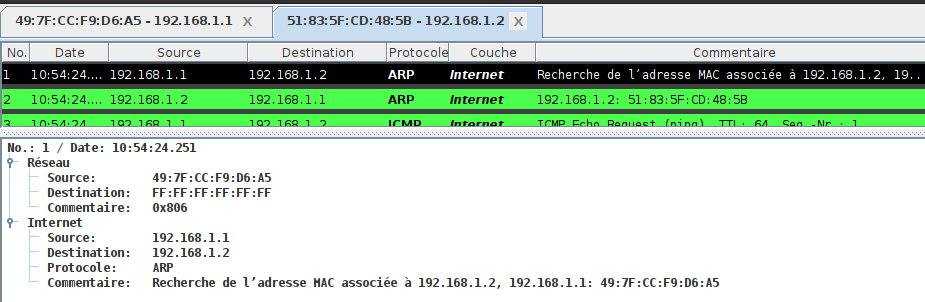
\includegraphics{images/arp1.png}\\

\begin{enumerate}
\def\labelenumi{\arabic{enumi}.}
\setcounter{enumi}{4}
\tightlist
\item
  Déplier le détail du second paquet de données et répondre aux mêmes
  questions.
\end{enumerate}

\end{activite}

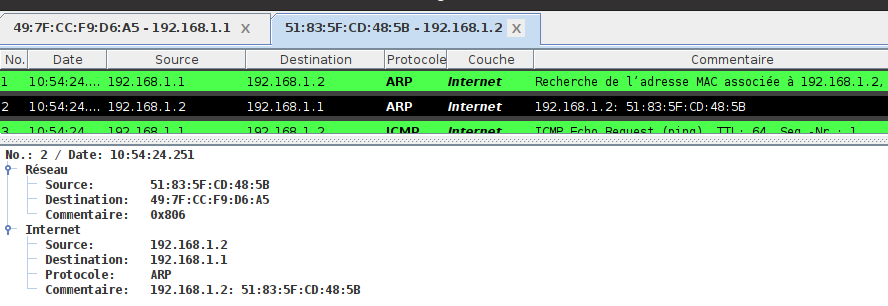
\includegraphics{images/arp2.png}\\

\begin{cours}{}

La couche \emph{liaison} du
\href{https://fr.wikipedia.org/wiki/Suite_des_protocoles_Internet}{modèle
TCP/IP} rassemble les protocoles permettant d'établir une connexion
physique directe, par la même technologie, de deux hôtes d'un même
réseau local (\textbf{LAN}).

Les protocoles les plus courants de cette couche sont
\href{https://fr.wikipedia.org/wiki/Ethernet}{Ethernet} pour une liaison
filaire et \href{https://fr.wikipedia.org/wiki/Wi-Fi}{Wifi} pour une
liaison par ondes.

Dans les deux cas, chaque hôte est identifié par une
\href{https://fr.wikipedia.org/wiki/Adresse_MAC}{adresse MAC}, parfois
nommée \textbf{adresse physique}. C'est un identifiant physique stocké
dans une carte réseau ou une interface réseau similaire. À moins qu'elle
n'ait été modifiée par l'utilisateur, elle est unique au monde.

Elle est constitué de \(48\) bits réparties en \(6\) octets représentés
en notation hexadécimale et séparés par le caractère
\passthrough{\lstinline!:!} comme par exemple
\passthrough{\lstinline!fc:f8:ae:31:cb:67!}.

Les hôtes d'un même réseau
\href{https://fr.wikipedia.org/wiki/Ethernet}{Ethernet} (clients ou
serveurs), sont reliés par une sorte de multiprise appelée
\textbf{commutateur} ou \textbf{switch}, capable d'identifier
l'\href{https://fr.wikipedia.org/wiki/Adresse_MAC}{adresse MAC} de
l'hôte relié à l'une de ses prises.

Le protocole
\href{https://fr.wikipedia.org/wiki/Address_Resolution_Protocol}{ARP}
permet à un hôte émetteur de découvrir
l'\href{https://fr.wikipedia.org/wiki/Adresse_MAC}{adresse MAC} de son
destinataire, à travers la diffusion d'une demande en
\href{https://fr.wikipedia.org/wiki/Broadcast_(informatique)}{brodacast},
dénotée par l'adresse \passthrough{\lstinline!FF:FF:FF:FF:FF:FF!} à
l'ensemble des hôtes du réseau local.

\end{cours}

\begin{exercice}{}

\emph{QCM type E3C}

Parmi les adresses suivantes, laquelle est une adresse Ethernet non
valide ?

\begin{itemize}
\tightlist
\item
  \textbf{Réponse A :} 8D:A9:D5:67:E6:F3
\item
  \textbf{Réponse B :} 8d:a9:d5:67:e6:f3
\item
  \textbf{Réponse C :} 8H:A9:D5:67:E6:F3
\item
  \textbf{Réponse D :} FF:A9:D5:67:E6:F3
\end{itemize}

\end{exercice}

\hypertarget{la-couche-ruxe9seau-ou-internet-du-moduxe8le-tcpip}{%
\subsection{La couche réseau, ou internet, du modèle
TCP/IP}\label{la-couche-ruxe9seau-ou-internet-du-moduxe8le-tcpip}}

\begin{figure}
\centering
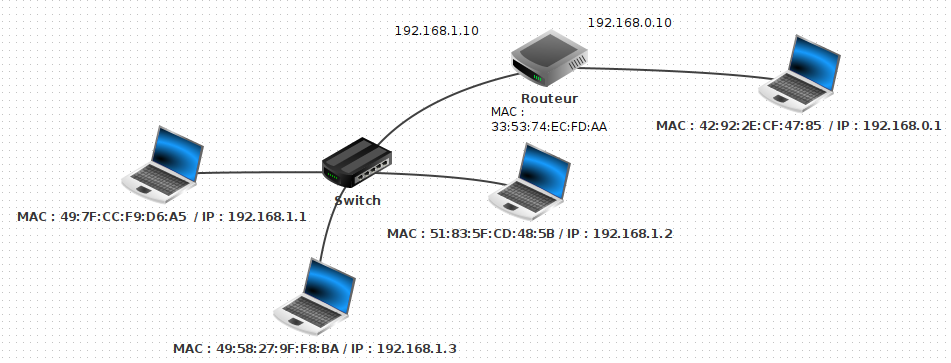
\includegraphics{images/wlan1.png}
\caption{Une interconnexion de réseau avec un routeur}
\end{figure}

\begin{activite}{}

\begin{enumerate}
\def\labelenumi{\arabic{enumi}.}
\item
  Ouvrir avec le logiciel
  \href{https://www.lernsoftware-filius.de/Herunterladen}{Filius} le
  fichier \passthrough{\lstinline!wlan1.fls!}. Quels sont les
  équipements présents dans ce réseau ? Sélectionner le mode
  \emph{construction}
  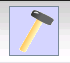
\includegraphics[width=0.1\textwidth,height=\textheight]{images/filius-construction.png}~Faire
  un clic droit sur chacune des machines du réseau, sélectionner
  \emph{Configurer} et noter leurs adresse IP. Il s'agit d'un
  identifiant de 32 bits constitué de quatre octets notés en base dix
  (valeurs entre 0 et 255) séparés par le symbole
  \passthrough{\lstinline!.!}
\item
  Sélectionner le mode \emph{simulation}
  
\includegraphics[width=0.1\textwidth,height=\textheight]{images/filius-simulation.png}~
  Faire un clic droit sur la machine d'adresse IP
  \passthrough{\lstinline!192.168.1.1!} pour afficher le bureau, ouvrir
  une fenêtre de ligne de commandes et saisir la commande
  \passthrough{\lstinline!ping 192.168.0.1!} qui envoie successivement
  quatre paquets de données pour tester la liaison avec la machine
  d'adresse IP \passthrough{\lstinline!192.168.0.1!}. Sélectionner
  l'affichage des échanges de données avec un clic droit sur la machine
  \passthrough{\lstinline!192.168.0.1!}.
\item
  Pour les quatre premiers paquets de données échangées, noter les
  adresses MAC et IP de l'émetteur et du destinataire et déterminer la
  fonction de chaque message.
\end{enumerate}

\begin{enumerate}
\def\labelenumi{\arabic{enumi}.}
\setcounter{enumi}{3}
\item
  Recommencer l'opération mais en testant la liaison entre les hôtes
  \passthrough{\lstinline!192.168.1.1!} et
  \passthrough{\lstinline!192.168.1.2!}. Quelles différences peut-on
  noter ?
\item
  Dans une interconnexion de réseau, chaque interface est identifiée de
  façon unique par son adresse IP. Les adresses IP de la forme
  \passthrough{\lstinline!192.168.1.X!} correspondent à des interfaces
  qui sont dans le même réseau local, les adresses IP de la forme
  \passthrough{\lstinline!192.168.0.X!} dénotent un autre réseau local.
  Ces deux réseaux sont interconnectés par un \textbf{routeur}.

  Quelle est la particularité du \textbf{routeur} ?

  Si on compare une interconnexion de réseau comme Internet au réseau
  postal, quelle analogie peut-on faire pour une adresse IP ?
\item
  Passer en mode construction et afficher les configurations des hôtes
  d'adresses IP \passthrough{\lstinline!192.168.1.1!} et
  \passthrough{\lstinline!192.168.0.1!}. Convertir en binaire les quatre
  entiers composant le masque et faire un ET logique bit à bit entre le
  masque et l'adresse IP de l'hôte. Quelle adresse IP obtient-on ?
\item
  Échanger les machines d'adresses MAC
  \passthrough{\lstinline!49:7F:CC:F9:D6:A5!} et
  \passthrough{\lstinline!42:92:2E:CF:47:85!}. En mode construction,
  permuter leurs configurations réseau : adresse IP et adresse de la
  passerelle. Tester la liaison avec la commande
  \passthrough{\lstinline!ping!}.

  D'après vous ,pourquoi désigne-t-on l'adresse MAC comme adresse
  physique et l'adresse IP comme adresse logique ?
\end{enumerate}

\end{activite}

\begin{center}

\begin{tabular}{cc}

\begin{minipage}{0.5\linewidth}

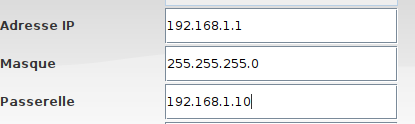
\includegraphics{images/config_passerelle.png}\\

\end{minipage} &

\begin{minipage}{0.5\linewidth}

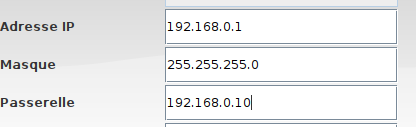
\includegraphics{images/config_passerelle2.png}\\

\end{minipage} \end{tabular}

\end{center}

\begin{figure}
\centering
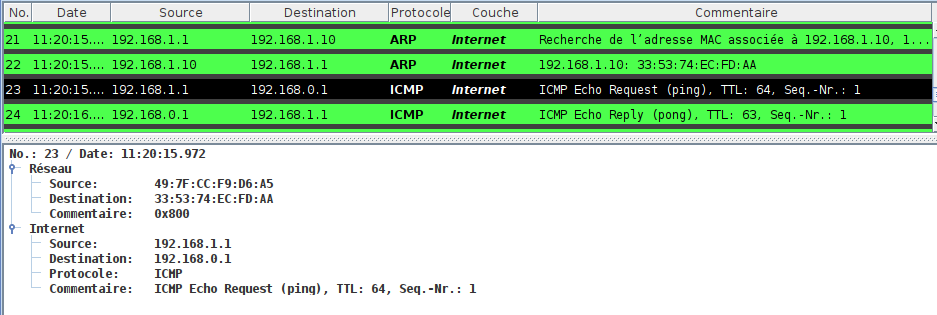
\includegraphics{images/ping_wlan.png}
\caption{Ping de 192.168.1.1 vers 192.168.0.1}
\end{figure}

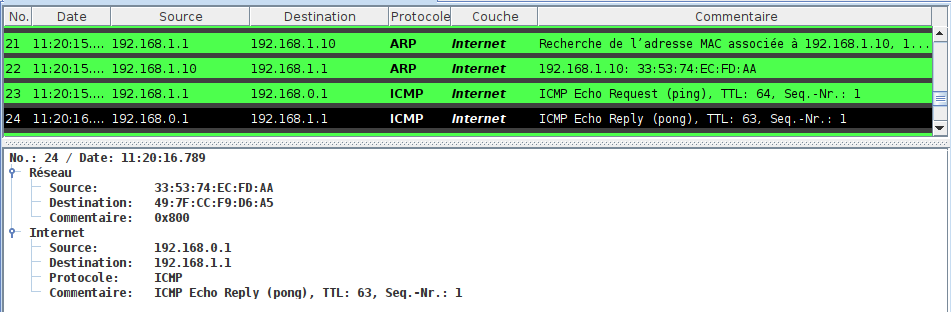
\includegraphics{images/pong_wlan.png}\\

\emph{Pong de 192.168.1.1 vers 192.168.0.1}

\begin{cours}{}

\begin{itemize}
\item
  Dans les années 1970,
  \href{https://fr.wikipedia.org/wiki/Vint_Cerf}{Vinton Cerf et Robert
  Kahn} en s'inspirant des travaux de
  \href{https://interstices.info/louis-pouzin-la-tete-dans-les-reseaux/}{Louis
  Pouzin}, ont développé le protocole
  \href{https://fr.wikipedia.org/wiki/Internet_Protocol}{Internet
  Protocol (IP)} qui permet d'interconnecter des réseaux locaux. C'est
  un protocole de la couche \emph{réseau} ou \emph{internet} dans le
  \href{https://fr.wikipedia.org/wiki/Suite_des_protocoles_Internet}{modèle
  en couches TCP/IP}.
\item
  La première fonctionnalité du protocole
  \href{https://fr.wikipedia.org/wiki/Internet_Protocol}{IP} est
  \emph{l'adressage}.

  \begin{itemize}
  \tightlist
  \item
    Chaque interface d'une machine hôte de l'interconnexion de réseaux
    reçoit un identifiant unique appelé \textbf{adresse IP}. Dans la
    version 4 du protocole, elle est représentée sur 32 bits par 4
    octets notés en décimal séparés par des points. Selon le principe
    d'\textbf{encapsulation des données}, les adresses
    \href{https://fr.wikipedia.org/wiki/Internet_Protocol}{IP} de
    l'émetteur et du destinataire du message sont ajoutés dans
    \emph{l'entête}
    \href{https://fr.wikipedia.org/wiki/Internet_Protocol}{IP}.
  \end{itemize}

  \href{https://commons.wikimedia.org/wiki/File:Addresse_Ipv4.svg}{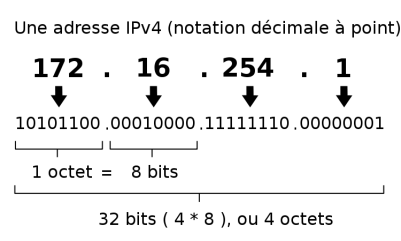
\includegraphics[width=0.6\textwidth,height=\textheight]{images/750px-Addresse_Ipv4_svg.png}}

  \begin{itemize}
  \tightlist
  \item
    L'adresse \href{https://fr.wikipedia.org/wiki/Internet_Protocol}{IP}
    est une \textbf{adresse logique}, elle n'est pas attachée
    définitivement à une machine, elle peut changer si la machine est
    déplacée dans un autre réseau. De plus une adresse
    \href{https://fr.wikipedia.org/wiki/Internet_Protocol}{IP} dénote
    une interface réseau et une machine, comme un \textbf{routeur}, peut
    en posséder plusieurs.
  \item
    Il existe des adresses
    \href{https://fr.wikipedia.org/wiki/Internet_Protocol}{IP} spéciales
    comme \passthrough{\lstinline!127.0.0.1!} qui correspond à la
    machine elle-même.
  \end{itemize}
\item
  La seconde fonctionnalité du protocole
  \href{https://fr.wikipedia.org/wiki/Internet_Protocol}{IP} est
  \emph{le routage} des paquets de données à travers différents réseaux
  locaux.

  \begin{itemize}
  \tightlist
  \item
    Un \textbf{routeur} est un équipement situés à la frontière d'au
    moins deux réseaux, possédant une interface dans (et donc au moins
    deux adresses IP) et qui joue le rôle de \textbf{passerelle} entre
    les deux.
  \item
    En pratique un émetteur envoie un paquet de données directement à
    son destinataire (en passant par un \textbf{switch}) s'il est sur le
    même réseau local et sinon il le transmet à sa \textbf{passerelle}.
    Celle-ci peut le transmettre directement si elle est connectée au
    réseau du destinataire sinon elle l'envoie à une autre
    \textbf{passerelle}.
  \item
    De proche en proche et grâce à des \emph{algorithmes de routage}, le
    message parvient jusqu'au destinataire. Chaque \textbf{passerelle}
    possède des \emph{tables de routage} pour déterminer le prochain
    saut dans la transmission d'un message reçu.
  \item
    Tous les paquets de données transmis d'un hôte émetteur vers un
    destinataire ne suivent pas forcément le même chemin. Si la
    topologie physique de l'interconnexion de réseaux évolue (routeurs
    ajoutés, enlevés, en panne) ou si le traffic est trop important sur
    certains liens, les routeurs intermédiaires vont dynamiquement
    mettre à jour leurs \emph{tables de routages} et peuvent changer le
    routage de paquets avec le même couple (émetteur, destinataires).
    C'est le principe de la \textbf{commutation de paquets}.
  \item
    Une \emph{configuration réseau} permet à un hôte émetteur de
    déterminer si le destinataire d'un message fait partie du même
    réseau local. Cette configuration est constituée :

    \begin{itemize}
    \tightlist
    \item
      de l'adresse
      \href{https://fr.wikipedia.org/wiki/Internet_Protocol}{IP} de
      l'interface
    \item
      de l'adresse
      \href{https://fr.wikipedia.org/wiki/Internet_Protocol}{IP} de sa
      \textbf{passerelle}
    \item
      d'un \textbf{masque de sous-réseau} au format d'une adresse
      \href{https://fr.wikipedia.org/wiki/Internet_Protocol}{IP} qui
      permet de séparer les parties \emph{réseau} et \emph{hôte} dans
      une adresse
      \href{https://fr.wikipedia.org/wiki/Internet_Protocol}{IP}. Tous
      les hôtes d'un même réseau local partagent le même \emph{préfixe
      réseau}.
    \end{itemize}
  \item
    Une \emph{configuration réseau} peut être attribuée automatiquement
    par le service réseau
    \href{https://fr.wikipedia.org/wiki/Dynamic_Host_Configuration_Protocol}{DHCP}
    ou de façon statique dans un fichier de configuration.
  \end{itemize}
\end{itemize}

\end{cours}

\begin{methode}{}

Voici quelques exemples pour extraire le \emph{préfixe réseau} à partir
d'une adresse \href{https://fr.wikipedia.org/wiki/Internet_Protocol}{IP}
et d'un \textbf{masque de sous-réseau}. Il faut effectuer un \textbf{ET
logique} entre les représentations binaires de l'adresse
\href{https://fr.wikipedia.org/wiki/Internet_Protocol}{IP} et du
\textbf{masque de sous-réseau}.

\emph{Cette méthode est hors-programme pour le bac !}

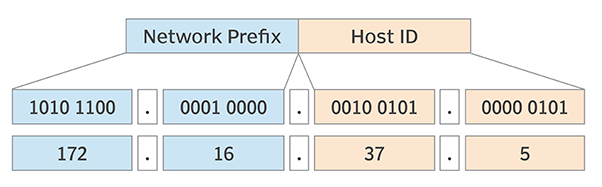
\includegraphics[width=0.5\textwidth,height=\textheight]{images/ip-subnet.png}\\

\begin{enumerate}
\def\labelenumi{\arabic{enumi}.}
\tightlist
\item
  Si le nombre de bits du \textbf{masque de sous-réseau} est un multiple
  de 8 : \passthrough{\lstinline!255.0.0.0!},
  \passthrough{\lstinline!255.255.0.0!}, ou
  \passthrough{\lstinline!255.255.255.0!} il suffit de masquer la partie
  de l'adresse
  \href{https://fr.wikipedia.org/wiki/Internet_Protocol}{IP}
  correspondant aux \passthrough{\lstinline!0!} du masque. Le passage en
  binaire n'est pas nécessaire.
\end{enumerate}

\begin{longtable}[]{@{}lll@{}}
\toprule
Adresse & Binaire & Décimal\tabularnewline
\midrule
\endhead
adresse IP & 00010111.10101000.00010111.00000010 &
192.168.23.2\tabularnewline
masque & 11111111.11111111.11111111.00000000 &
255.255.112.0\tabularnewline
adresse réseau & 11000000.10101000.00010111.00000000 &
192.168.23.0\tabularnewline
\bottomrule
\end{longtable}

\begin{enumerate}
\def\labelenumi{\arabic{enumi}.}
\setcounter{enumi}{1}
\tightlist
\item
  Sinon, le passage en binaire est nécessaire.
\end{enumerate}

\begin{longtable}[]{@{}lll@{}}
\toprule
Adresse & Binaire & Décimal\tabularnewline
\midrule
\endhead
adresse IP & 00010111.10101000.00010111.00000010 &
192.168.23.2\tabularnewline
masque & 11111111.11111111.11110000.00000000 &
255.255.112.0\tabularnewline
adresse réseau & 11000000.10101000.00010000.00000000 &
192.168.16.0\tabularnewline
\bottomrule
\end{longtable}

Un \textbf{masque de sous-réseau} peut être caractériser par sa longueur
en bits. La notation
\href{https://fr.wikipedia.org/wiki/Sous-r\%C3\%A9seau}{CIDR} est une
façon compacte d'ajouter cette information à la suite d'une adresse
\href{https://fr.wikipedia.org/wiki/Internet_Protocol}{IP} en les
séparant par le symbole \passthrough{\lstinline!/!}.

L'adresse du premier exemple sera ainsi notée
\passthrough{\lstinline!192.168.23.2/24!} et celle du second
\passthrough{\lstinline!192.168.23.2/20!}.

Pour s'entraîner on pourra utilise ce
\href{https://cric.grenoble.cnrs.fr/Administrateurs/Outils/CalculMasque/}{calculateur
en ligne}.

\end{methode}

\begin{exercice}{}

Donner les adresses réseau correspondant à ces adresses
\href{https://fr.wikipedia.org/wiki/Internet_Protocol}{IP} en notation
\href{https://fr.wikipedia.org/wiki/Sous-r\%C3\%A9seau}{CIDR} :
148.33.1.112/8 , 82.30.12.18/24 et 91.198.174.3/19

\end{exercice}

\begin{methode}{}

Quelques commandes réseau sont à connaître.

\begin{enumerate}
\def\labelenumi{\arabic{enumi}.}
\tightlist
\item
  La commande \passthrough{\lstinline!ping!} permet de tester la liaison
  avec un hôte si on connaît son adresse
  \href{https://fr.wikipedia.org/wiki/Internet_Protocol}{IP} ou son nom
  de domaine. On l'interrompt avec le signal envoyé par
  \passthrough{\lstinline!CTRL + C!}.
\end{enumerate}

\begin{lstlisting}[language=bash]
junier@fredportable:~$ ping 192.168.1.254
PING 192.168.1.254 (192.168.1.254) 56(84) bytes of data.
64 bytes from 192.168.1.254: icmp_seq=1 ttl=64 time=2.27 ms
64 bytes from 192.168.1.254: icmp_seq=2 ttl=64 time=3.83 ms
64 bytes from 192.168.1.254: icmp_seq=3 ttl=64 time=2.60 ms
^C
--- 192.168.1.254 ping statistics ---
9 packets transmitted, 9 received, 0% packet loss, time 8013ms
rtt min/avg/max/mdev = 2.184/3.020/4.642/0.844 ms
\end{lstlisting}

\begin{enumerate}
\def\labelenumi{\arabic{enumi}.}
\setcounter{enumi}{1}
\tightlist
\item
  Les commandes \passthrough{\lstinline!ifconfig!} ou
  \passthrough{\lstinline!ip address!} sous Linux ou
  \passthrough{\lstinline!ipconfig!} sous Windows permettent d'afficher
  les adresses physique (MAC) ou logiques (IP) d'une interface réseau.
  Par exemple l'adresse MAC de l'interface Wifi ci-dessous est
  \passthrough{\lstinline!fc:f8:ae:31:cb:67!} et son adresse IPV4, au
  moment de l'exécution, était \passthrough{\lstinline!192.168.1.98!}.
  On remarque un autre format IPV6 codé sur 128 bits en hexadécimal, mis
  en place progressivement pour faire face à la pénurie d'adresses IPV4
  sur 32 bits (soit \(2^{32}=4294967296\) adresses).
\end{enumerate}

\begin{lstlisting}[language=bash]
anonymous@laptop:~$ ifconfig
wlp2s0: flags=4163<UP,BROADCAST,RUNNING,MULTICAST>  mtu 1500
        inet 192.168.1.98  netmask 255.255.255.0  broadcast 192.168.1.255
        inet6 fe80::2d0d:7c56:cc75:cadb  prefixlen 64  scopeid 0x20<link>
        ether fc:f8:ae:31:cb:67  txqueuelen 1000  (Ethernet)
        RX packets 50800  bytes 45120378 (45.1 MB)
        RX errors 0  dropped 0  overruns 0  frame 0
        TX packets 37659  bytes 5251257 (5.2 MB)
\end{lstlisting}

\begin{enumerate}
\def\labelenumi{\arabic{enumi}.}
\setcounter{enumi}{2}
\tightlist
\item
  La commande \passthrough{\lstinline!route -n!} sous Linux permet
  d'afficher la passerelle et le masque de sous-réseau d'une interface.
  Ci-dessous l'adresse de l'hôte est
  \passthrough{\lstinline!192.168.1.0!}, celle de la passerelle
  \passthrough{\lstinline!192.168.1.254!} et le masque est
  \passthrough{\lstinline!255.255.255.0!}.
\end{enumerate}

\begin{lstlisting}[language=bash]
anonymous@laptop:~$ route -n
Table de routage IP du noyau
Destination     Passerelle      Genmask         Indic Metric Ref    Use Iface
0.0.0.0         192.168.1.254   0.0.0.0         UG    600    0        0 wlp2s0
192.168.1.0     0.0.0.0         255.255.255.0   U     600    0        0 wlp2s0
\end{lstlisting}

\begin{enumerate}
\def\labelenumi{\arabic{enumi}.}
\setcounter{enumi}{3}
\tightlist
\item
  La commande \passthrough{\lstinline!traceroute!} utilise le champ
  \href{https://fr.wikipedia.org/wiki/Time_to_Live}{TTL} de
  l'\emph{entête} IP pour tracer les routeurs sur le chemin entre un
  hôte émetteur et un destinataire dont on connaît l'adresse
  \href{https://fr.wikipedia.org/wiki/Internet_Protocol}{IP} ou le nom
  de domaine. Le nombre de sauts maximum est de 30.
\end{enumerate}

\begin{lstlisting}[language=bash]
anonymous@laptop:~$ traceroute qwant.com
traceroute to qwant.com (194.187.168.99), 30 hops max, 60 byte packets
 1  _gateway (192.168.1.254)  5.397 ms  5.415 ms  6.008 ms
 2  176-145-144-2.abo.bbox.fr (176.145.144.2)  29.450 ms  29.952 ms  31.584 ms
 3  212.194.170.233 (212.194.170.233)  38.825 ms  42.428 ms  43.469 ms
 4  be5.cbr01-ntr.net.bbox.fr (212.194.171.137)  44.712 ms  45.358 ms  46.831 ms
 5  * * *
 6  qwant.par.franceix.net (37.49.236.134)  48.854 ms  25.381 ms  25.308 ms
\end{lstlisting}

\end{methode}

\begin{exercice}{}

\emph{QCM type E3C}

\begin{enumerate}
\def\labelenumi{\arabic{enumi}.}
\tightlist
\item
  Laquelle de ces écritures ne désigne pas une adresse IP~?
\end{enumerate}

\begin{itemize}
\tightlist
\item
  \textbf{Réponse A :} 127.0.0.1
\item
  \textbf{Réponse B :} 207.142.131.245
\item
  \textbf{Réponse C :} 192.168.229.48
\item
  \textbf{Réponse D :} 296.141.2.4
\end{itemize}

\begin{enumerate}
\def\labelenumi{\arabic{enumi}.}
\setcounter{enumi}{1}
\tightlist
\item
  Sur la configuration IP d'une machine nommée MACH01 on peut lire~:
\end{enumerate}

adresse Ipv4~: 172.16.100.201 Masque de sous-réseau~: 255.255.0.0
Passerelle~: 172.16.0.254

Sur la configuration IP d'une machine nommée MACH02 on peut lire~:

adresse Ipv4~: 172.16.100.202 Masque de sous-réseau~: 255.255.0.0
Passerelle~: 172.16.0.254

Depuis la machine MACH02, à l'aide de quelle commande peut-on tester le
dialogue entre ces deux machines~?

\begin{itemize}
\tightlist
\item
  \textbf{Réponse A :} ping 172.16.100.201
\item
  \textbf{Réponse B :} ping 172.16.100.202
\item
  \textbf{Réponse C :} ping 172.16.100.254
\item
  \textbf{Réponse D :} ping 255.255.0.0
\end{itemize}

\begin{enumerate}
\def\labelenumi{\arabic{enumi}.}
\setcounter{enumi}{2}
\tightlist
\item
  Dans un terminal sous Linux, à quoi sert la commande traceroute ?
\end{enumerate}

\begin{itemize}
\tightlist
\item
  \textbf{Réponse A :} à afficher un itinéraire routier entre deux
  villes
\item
  \textbf{Réponse B :} c'est un synonyme pour la commande ping
\item
  \textbf{Réponse C :} à afficher le chemin suivi par des paquets à
  travers un protocole IP
\item
  \textbf{Réponse D :} à suivre pas à pas l'exécution d'un programme
\end{itemize}

\begin{enumerate}
\def\labelenumi{\arabic{enumi}.}
\setcounter{enumi}{3}
\tightlist
\item
  Quelle est l'utilité de la commande ping dans un réseau informatique ?
\end{enumerate}

\begin{itemize}
\tightlist
\item
  \textbf{Réponse A :} établir un réseau privé virtuel
\item
  \textbf{Réponse B :} tester si la connexion peut être établie avec une
  machine distante
\item
  \textbf{Réponse C :} obtenir la route suivie par un paquet dans le
  réseau
\item
  \textbf{Réponse D :} mesurer les performances d'une machine distante
\end{itemize}

\begin{enumerate}
\def\labelenumi{\arabic{enumi}.}
\setcounter{enumi}{4}
\tightlist
\item
  Quel matériel permet d'interconnecter des \textbf{réseaux} entre eux :
\end{enumerate}

\begin{itemize}
\tightlist
\item
  \textbf{Réponse A :} un routeur
\item
  \textbf{Réponse B :} un commutateur (ou \emph{switch})
\item
  \textbf{Réponse C :} un interconnecteur
\item
  \textbf{Réponse D :} un serveur
\end{itemize}

\begin{enumerate}
\def\labelenumi{\arabic{enumi}.}
\setcounter{enumi}{5}
\tightlist
\item
  Quel protocole permet d'attribuer dynamiquement une adresse IP ?
\end{enumerate}

\begin{itemize}
\tightlist
\item
  \textbf{Réponse A :} UDP
\item
  \textbf{Réponse B :} HTTP
\item
  \textbf{Réponse C :} DHCP
\item
  \textbf{Réponse D :} DNS
\end{itemize}

\end{exercice}

\hypertarget{la-couche-transport-du-moduxe8le-tcpip}{%
\subsection{La couche transport du modèle
TCP/IP}\label{la-couche-transport-du-moduxe8le-tcpip}}

\begin{figure}
\centering
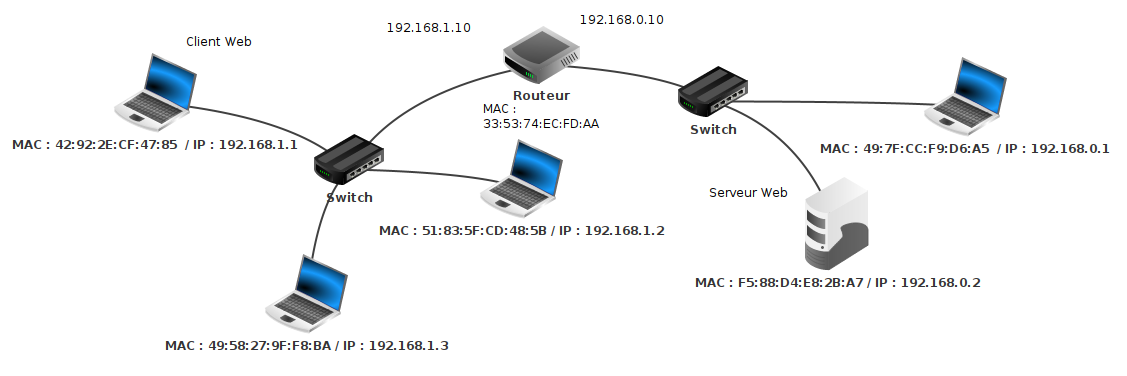
\includegraphics{images/wlan3.png}
\caption{Réseau avec serveur Web}
\end{figure}

\begin{activite}{}

\begin{enumerate}
\def\labelenumi{\arabic{enumi}.}
\tightlist
\item
  Ouvrir avec le logiciel
  \href{https://www.lernsoftware-filius.de/Herunterladen}{Filius} le
  fichier \passthrough{\lstinline!wlan3.fls!}. Il s'agit du même réseau
  que dans \passthrough{\lstinline!wlan3.fls!} avec un ordinateur
  d'adresse IP \passthrough{\lstinline!192.168.0.2!}et un switch en plus
  dans le réseau d'adresse \passthrough{\lstinline!192.168.0.0!}.
\item
  Sélectionner le mode \emph{simulation}
  
\includegraphics[width=0.1\textwidth,height=\textheight]{images/filius-simulation.png}~
  Faire un clic droit sur la machine d'adresse IP
  \passthrough{\lstinline!192.168.0.2!}, afficher le bureau, installer
  un serveur Web et le démarrer. Faire un clic droit sur la machine
  d'adresse IP \passthrough{\lstinline!192.168.1.1!}, , afficher le
  bureau, installer un navigateur Web et saisir dans la barre d'adresse
  \passthrough{\lstinline!http://192.168.0.2!} pour envoyer une requête
  HTTP demandant la page d'accueil du serveur Web sur
  \passthrough{\lstinline!192.168.0.2!}. Afficher les données échangées,
  on devrait obtenir l'historique ci-dessous.
\item
  La requête HTTP est-elle le premier paquet de données échangé ?
\end{enumerate}

\end{activite}

\begin{figure}
\centering
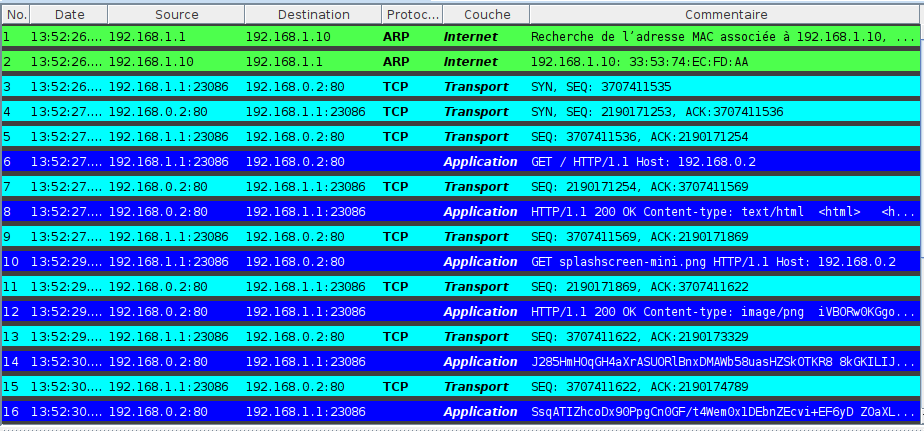
\includegraphics{images/filius-tcp1.png}
\caption{Requête HTTP avec une adresse IP}
\end{figure}

\begin{cours}{}

\begin{itemize}
\item
  Le protocole
  \href{https://fr.wikipedia.org/wiki/Internet_Protocol}{IP} de la
  couche \emph{réseau} permet la transmission d'un paquet de données
  entre deux machines hôtes. Il s'exécute sur tous les routeurs
  traversés lors du chemin. Néanmoins, plusieurs services réseaux
  peuvent s'exécuter sur l'émetteur et le destinataire. Pour faire
  communiquer deux programes, il faut donc un paramètre d'adresse
  supplémentaire, appelé \textbf{port}.
\item
  Les protocoles
  \href{https://fr.wikipedia.org/wiki/Transmission_Control_Protocol}{TCP}
  et \href{https://fr.wikipedia.org/wiki/User_Datagram_Protocol}{UDP} de
  la couche \emph{transport} encapsulent un paquet IP à émettre avec un
  \emph{entête} contenant les numéros de \textbf{port} des appplications
  chez émetteur et le destinataire. Ces protocoles s'exécutent de
  \emph{bout en bout} sur l'émetteur et le destinataire mais pas sur les
  routeurs intermédiaires.
\item
  D'après le principe de \textbf{multiplexage}, les données sont
  découpées en paquets qui sont transmis séparément sur le réseau et qui
  peuvent suivre des chemins différents et donc se perdre ou arriver
  dans le désordre d'après le principe de \textbf{commutation de
  paquets}. Cette souplesse du
  \href{https://fr.wikipedia.org/wiki/Suite_des_protocoles_Internet}{modèle
  TCP/IP} est la clef du succès d'Internet mais elle nécessite des
  mécanismes pour garantir la \emph{fiabilité} des transmissions :
  ordonner les paquets, demander la réémission de paquets perdus
  \ldots{}
\item
  Le protocole
  \href{https://fr.wikipedia.org/wiki/User_Datagram_Protocol}{UDP}
  fonctionne en mode non connecté et n'offre pas ces services car il est
  utilisé dans des applications avec des questions/réponses simples
  (\href{https://fr.wikipedia.org/wiki/Domain_Name_System}{DNS} ) ou
  pour lesquelles les erreurs de transmission ne sont pas critiques et
  qui ont besoin de rapidité (streaming video, jeu en ligne \ldots).
\item
  Le protocole
  \href{https://fr.wikipedia.org/wiki/Transmission_Control_Protocol}{TCP}
  établit une connexion entre l'émetteur et le destinataire et résout
  les problèmes de qualité de service grâce à un système d'\emph{accusés
  de réception}.
\end{itemize}

\end{cours}

\begin{center}

\begin{tabular}{cc}

\begin{minipage}{0.5\linewidth}

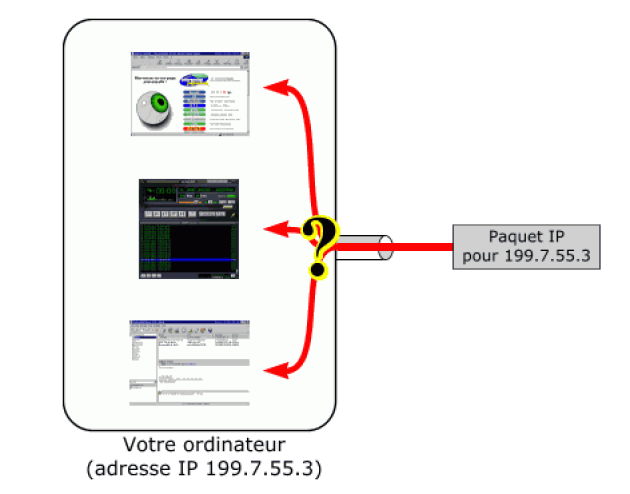
\includegraphics{images/UDP1.png}\\

\end{minipage} &

\begin{minipage}{0.5\linewidth}

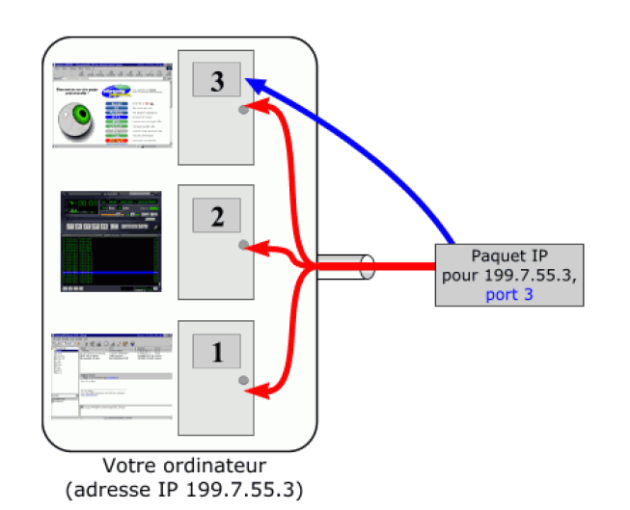
\includegraphics{images/UDP2.png}\\

\end{minipage} \end{tabular}

\end{center}

\begin{methode}{}

Expliquons le fonctionnement du protocole
\href{https://fr.wikipedia.org/wiki/Transmission_Control_Protocol}{TCP}
à partir de l'historique d'échanges de la figure 12.

\emph{La connaissance de TCP est hors-programme mais nous étudierons en
dernière partie un protocole simplifié de récupération de paquets qui
est au programme !}

\begin{enumerate}
\def\labelenumi{\arabic{enumi}.}
\item
  Pour établir une \emph{connexion TCP} entre un émetteur et un
  destinataire, les deux hôtes procèdent à un partage de numéros de
  séquences des paquets de données qu'ils vont transmettre lors d'une
  phase de trois échanges nommée
  \href{https://fr.wikipedia.org/wiki/Three-way_handshake}{three
  handshake} (voir figure 13). Elle correspond aux échanges 3, 4 et 5 de
  la figure 12 :

  \begin{itemize}
  \tightlist
  \item
    Le client d'IP \passthrough{\lstinline!192.168.1.1!} envoie un
    paquet avec le drapeau \passthrough{\lstinline!SYN!} et un numéro de
    séquence SEQ 3707411535 qu'il a choisi.
  \item
    Le serveur \passthrough{\lstinline!192.168.0.2!} lui répond avec un
    paquet de drapeau\passthrough{\lstinline!SYN!} qui contient un
    numéro de séquence SEQ 2190171253 qu'il a choisi et un numéro
    d'acquittement \passthrough{\lstinline!ACK!} avec le numéro de la
    prochaine séquence d'octets attendu de
    \passthrough{\lstinline!192.168.1.1!}.
  \item
    Le client \passthrough{\lstinline!192.168.1.1!} confirme avec un
    paquet sans drapeau qui contient le numéro de séquence
    \passthrough{\lstinline!SEQ!} correspondant au dernier numéro
    d'acquittement \passthrough{\lstinline!ACK!} reçu et un
    \passthrough{\lstinline!ACK!} indiquant au serveur le numéro de
    séquence du prochain paquet attendu.
  \end{itemize}
\item
  Une fois la connexion ouverte, chaque message reçu est suivi par
  l'envoi d'un \emph{accusé de réception} (échanges de numéros impairs
  dans la figure 12) avec un numéro de séquence
  \passthrough{\lstinline!SEQ!} correspondant au dernier numéro
  d'acquittement \passthrough{\lstinline!ACK!} reçu et un accusé de
  réception indiquant à l'interlocuteur le numéro de séquence attendu
  lors de son prochain envoi : il se calcul en ajoutant à
  l'\passthrough{\lstinline!ACK!} précédent la taille du paquet qui
  vient d'être reçu. Ainsi chaque interlocuteur peut vérifier si son
  dernier paquet a été bien reçu (et le renvoyer éventuellement au bout
  d'un certain temps) et ordonner les paquets s'ils sont arrivés dans le
  désordre.
\item
  Toute connexion
  \href{https://fr.wikipedia.org/wiki/Transmission_Control_Protocol}{TCP}
  se termine par un \passthrough{\lstinline!handshaking!} en quatre de
  temps avec un échange de paquets marqués par le drapeau
  \passthrough{\lstinline!FIN!} (voir figure 14)
\end{enumerate}

\end{methode}

\begin{figure}
\centering
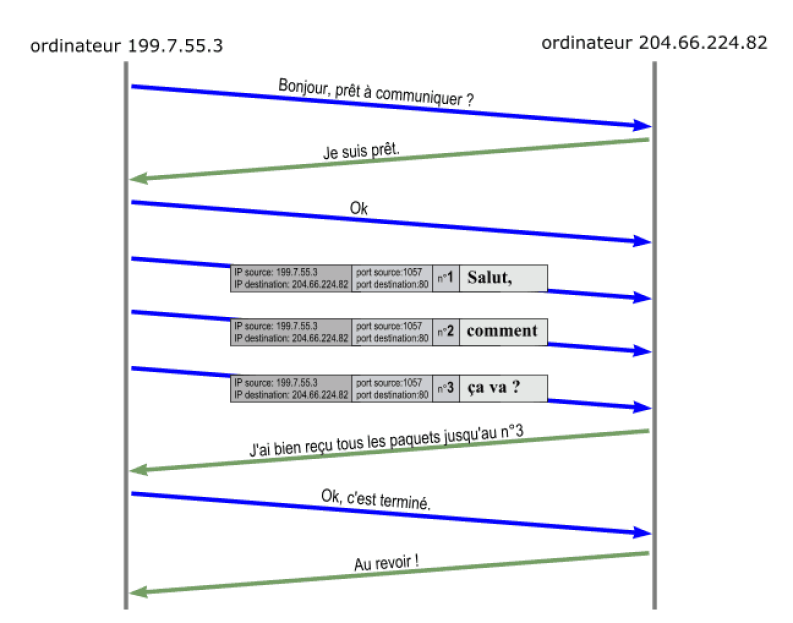
\includegraphics[width=0.8\textwidth,height=\textheight]{images/TCP1.png}
\caption{Ouverture d'une connexion TCP}
\end{figure}

\begin{figure}
\centering
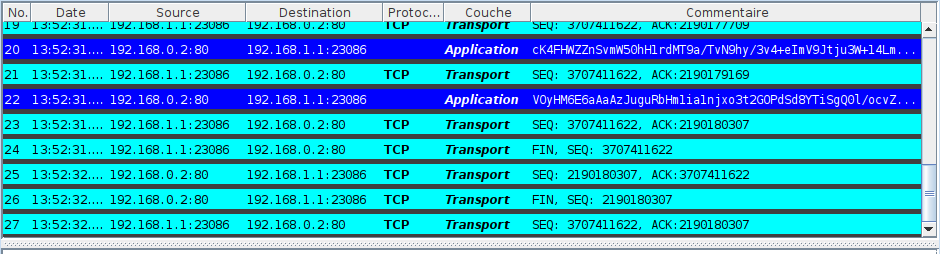
\includegraphics[width=1\textwidth,height=\textheight]{images/filius-tcp2.png}
\caption{Fin d'une connexion TCP}
\end{figure}

\begin{exercice}{}

\emph{QCM type E3C}

Dans le protocole de communication IP~:

\begin{itemize}
\tightlist
\item
  \textbf{Réponse A :} Les données sont envoyées en une seule partie.
\item
  \textbf{Réponse B :} Les données sont envoyées en plusieurs parties
  qui suivent le même itinéraire au sein du réseau.
\item
  \textbf{Réponse C :} Les données sont envoyées en plusieurs parties
  qui suivent des itinéraires différents au sein du réseau et arrivent à
  destination en respectant l'ordre de leur envoi.
\item
  \textbf{Réponse D :} Les données sont envoyées en plusieurs parties
  qui suivent des itinéraires différents au sein du réseau et arrivent à
  destination dans un ordre quelconque.
\end{itemize}

\end{exercice}

\hypertarget{la-couche-application-du-moduxe8le-tcpip}{%
\subsection{La couche application du modèle
TCP/IP}\label{la-couche-application-du-moduxe8le-tcpip}}

\begin{figure}
\centering
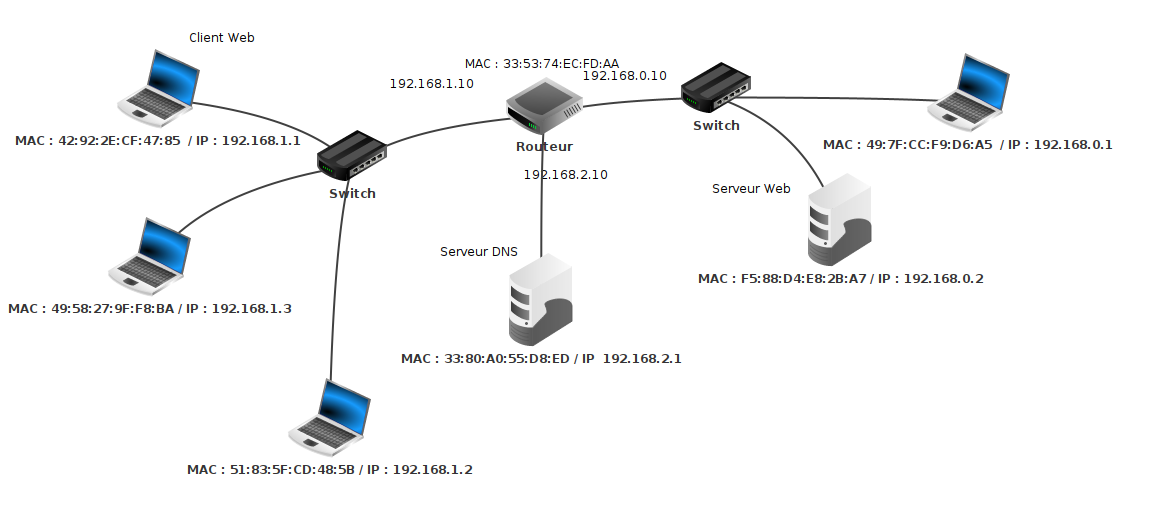
\includegraphics[width=1\textwidth,height=\textheight]{images/filius-dns.png}
\caption{Réseaux avec serveur DNS}
\end{figure}

\begin{activite}{}

\begin{enumerate}
\def\labelenumi{\arabic{enumi}.}
\tightlist
\item
  Ouvrir avec le logiciel
  \href{https://www.lernsoftware-filius.de/Herunterladen}{Filius} le
  fichier \passthrough{\lstinline!wlan4.fls!}. Par rapport aux réseaux
  de \passthrough{\lstinline!wlan3.fls!}, on a rajouté une interface
  \passthrough{\lstinline!192.168.2.10!} sur le routeur qui est
  connectée à un réseau local constitué d'une seule machine hôte
  d'adresse \passthrough{\lstinline!192.168.2.1!}.
\end{enumerate}

En pratique, on n'interroge pas un serveur Web avec son adresse
\href{https://fr.wikipedia.org/wiki/Internet_Protocol}{IP} mais avec un
\emph{nom de domaine}. Pour associer l'adresse
\href{https://fr.wikipedia.org/wiki/Internet_Protocol}{IP}
\passthrough{\lstinline!192.168.0.1!} du serveur Web au nom de domaine
\passthrough{\lstinline!www.monsite.org!}\}, on va rajouter un serveur
\href{https://fr.wikipedia.org/wiki/Domain_Name_System}{DNS} sur la
machine \passthrough{\lstinline!192.168.2.1!}.

\begin{enumerate}
\def\labelenumi{\arabic{enumi}.}
\setcounter{enumi}{1}
\item
  En mode construction, paramétrer le serveur
  \href{https://fr.wikipedia.org/wiki/Domain_Name_System}{DNS} sur la
  machine \passthrough{\lstinline!192.168.1.1!} avec l'adresse
  \passthrough{\lstinline!192.168.2.1!}.
\item
  En mode simulation, faire un clic droite sur la machine
  \passthrough{\lstinline!192.168.2.1!}, installer l'application serveur
  DNS, ajouter la règle de résolution du nom de domaine
  \passthrough{\lstinline!www.monsite.org!} par l'adresse
  \href{https://fr.wikipedia.org/wiki/Internet_Protocol}{IP} du serveur
  Web et démarrer le serveur
  \href{https://fr.wikipedia.org/wiki/Domain_Name_System}{DNS}.
\item
  Toujours en mode simulation, depuis la machine
  \passthrough{\lstinline!192.168.1.1!}, afficher le bureau, ouvrir le
  navigateur Web et saisir dans la barre d'adresse
  l'\href{https://fr.wikipedia.org/wiki/Uniform_Resource_Locator}{URL}
  \url{http://www.monsite.org}. Afficher les échanges de données, on
  doit obtenir un historique similaire à celui de la figure 16. Comparer
  avec l'historique de la figure 12 où le serveur Web avait été atteint
  à partir de son adresse IP. Quels paquets de données supplémentaires
  ont été echangés ? Entre quelles machines ? Quel est leur rôle ?
\end{enumerate}

\end{activite}

\begin{figure}
\centering
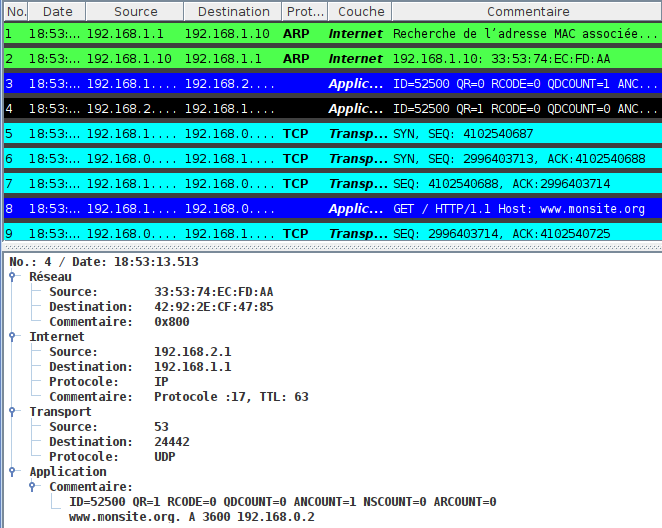
\includegraphics{images/filius-dns4.png}
\caption{Requête HTTP avec une URL}
\end{figure}

\begin{cours}{}

\begin{itemize}
\tightlist
\item
  La \emph{couche application} fournit des services permettant aux
  applications de l'utilisateur d'utiliser le réseau .
\item
  Ces programmes et les protocoles qu'ils utilisent incluent
  \href{https://fr.wikipedia.org/wiki/Hypertext_Transfer_Protocol}{HTTP}
  (Web),
  \href{https://fr.wikipedia.org/wiki/File_Transfer_Protocol}{FTP}
  (transfert de fichiers),
  \href{https://fr.wikipedia.org/wiki/Simple_Mail_Transfer_Protocol}{SMTP}(messagerie),
  \href{https://fr.wikipedia.org/wiki/Secure_Shell}{SSH}(connexion à
  distance sécurisée) ou
  \href{https://fr.wikipedia.org/wiki/Domain_Name_System}{DNS}
  (recherche de correspondance entre noms et adresses IP) \ldots{}
\item
  Ils sont souvent associés à des \textbf{ports}
  \href{https://fr.wikipedia.org/wiki/Transmission_Control_Protocol}{TCP}
  particuliers : 80 pour
  \href{https://fr.wikipedia.org/wiki/Hypertext_Transfer_Protocol}{HTTP},
  22 pour \href{https://fr.wikipedia.org/wiki/Secure_Shell}{SSH}
  \ldots{}
\end{itemize}

\end{cours}

\begin{methode}{}

\emph{Pour le bac il faut juste savoir que DNS est le service de
résolution de noms de domaines des URL en adresses IP.}

\begin{itemize}
\item
  Le \href{https://fr.wikipedia.org/wiki/Domain_Name_System}{DNS} , pour
  \emph{Domain Name System}, fait le lien entre les adresses
  \href{https://fr.wikipedia.org/wiki/Internet_Protocol}{IP} utilisées
  pour acheminer les paquets et les noms de machine utilisés par les
  utilisateurs ou les applications. Les noms de domaine figurent en
  particulier dans les
  \href{https://fr.wikipedia.org/wiki/Uniform_Resource_Locator}{URL} qui
  permettent de localiser les ressources dans l'hypertexte du Web. Par
  exemple dans
  l'\href{https://fr.wikipedia.org/wiki/Uniform_Resource_Locator}{URL}
  \url{https://fst-mathematiques.univ-lyon1.fr/formation/}, le nom de
  domaine est \passthrough{\lstinline!fst-mathematiques.univ-lyon1.fr!}.
  Les noms de domaines sont hiérarchisés dans une structure
  arborescente. Dans un nom de domaine, les domaines imbriqués sont
  séparés par un point : dans
  \passthrough{\lstinline!fst-mathematiques.univ-lyon1.fr!}, on a
  fst-mathematiques sous-domaine de univ-lyon1 sous-domaine de domaine
  de \passthrough{\lstinline!fr!} qui est un domaine de premier niveau
  ou Top Level Domain.
\item
  Le préfixe \passthrough{\lstinline!www!} qui apparaît souvent dans les
  URL du Web, désigne un sous-domaine particulier correspondant au
  répertoire public par défaut sur le serveur Web. Il n'est pas
  nécessaire dans
  l'\href{https://fr.wikipedia.org/wiki/Uniform_Resource_Locator}{URL}.
\item
  Les correspondances entre noms de domaine et adresses IP sont
  déterminées en interrogeant des serveurs
  \href{https://fr.wikipedia.org/wiki/Domain_Name_System}{DNS}(avec le
  protocole
  \href{https://fr.wikipedia.org/wiki/Domain_Name_System}{DNS}\ldots) .
  Chaque hôte sur internet est paramétré avec un serveur DNS par défaut.
  Un seul serveur DNS ne pouvant pas connaître toutes les adresses IP,
  DNS est un système distribué : chaque hôte possède un serveur DNS par
  défaut qui connaît l'adresse de serveurs racines qui eux-mêmes
  connaissent les adresses de serveurs DNS administrant les domaines de
  premier niveau. Pour résoudre un domaine, le serveur DNS de l'hôte
  procède par interrogations successives jusqu'à atteindre un serveur
  DNS détenant l'adresse IP du domaine recherché.
\item
  Les commandes \passthrough{\lstinline!host!} ou
  \passthrough{\lstinline!nslookup!} permettent sous Linux de résoudre
  des noms de domaines :
\end{itemize}

\begin{lstlisting}[language=bash]
junier@fredportable:~$ host qwant.com
qwant.com has address 194.187.168.99
qwant.com mail is handled by 50 mail1.qwant.com.
qwant.com mail is handled by 90 mail2.qwant.com.
junier@fredportable:~$ nslookup qwant.com
Server:     127.0.0.53
Address:    127.0.0.53#53

Non-authoritative answer:
Name:   qwant.com
Address: 194.187.168.99
\end{lstlisting}

\end{methode}

\begin{figure}
\centering
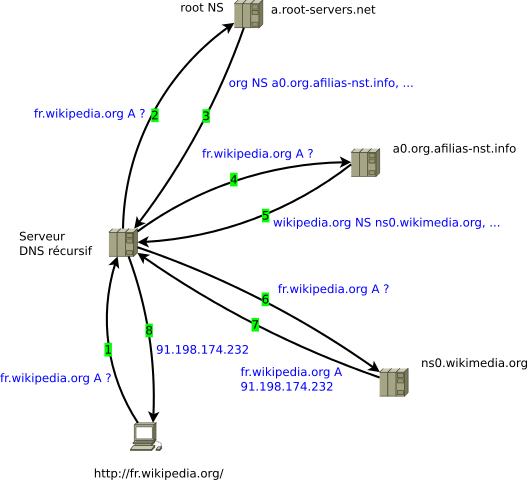
\includegraphics[width=0.6\textwidth,height=\textheight]{images/528px-DNS_iterations.svg.png}
\caption{Requêtes DNS itératives (source Wikipedia)}
\end{figure}

\begin{exercice}{}

\emph{QCM type E3C}

L'adresse IP du site \passthrough{\lstinline!www.education.gouv.fr!} est
185.75.143.24.

Quel dispositif permet d'associer l'adresse IP et l'URL
\passthrough{\lstinline!www.education.gouv.fr!} ?

\begin{itemize}
\tightlist
\item
  \textbf{Réponse A :} un routeur.
\item
  \textbf{Réponse B :} un serveur DNS.
\item
  \textbf{Réponse C :} un serveur de temps.
\item
  \textbf{Réponse D :} un serveur Web.
\end{itemize}

\end{exercice}

\hypertarget{uxe9tude-dun-protocole-de-ruxe9cupuxe9ration-de-paquet}{%
\section{Étude d'un protocole de récupération de
paquet}\label{uxe9tude-dun-protocole-de-ruxe9cupuxe9ration-de-paquet}}

\hypertarget{le-protocole-du-bit-alternuxe9}{%
\subsection{Le protocole du bit
alterné}\label{le-protocole-du-bit-alternuxe9}}

\emph{Le contenu de cette partie est directement inspiré des cours de
\href{http://archives.janviercommelemois.fr/nsi/fichiers_pdf/feuille-internet.pdf}{Romain
Janvier} ou
\href{https://pixees.fr/informatiquelycee/n_site/nsi_prem.html}{David
Roche}, merci à eux.}

\begin{cours}{}

\begin{itemize}
\item
  Le \textbf{protocole de bit alterné} était implémenté au niveau de la
  \emph{couche liaison} du modèle OSI. Le principe est simple :
  considérons 2 machines en réseau : une machine A, l'émetteur et une
  machine B, le destinataire. Lors de l'émission d'un paquet de données,
  A y ajoute un \emph{bit} (1 ou 0) appelé \emph{bit de contrôle}. À
  réception, B envoie un \emph{accusé de réception} (acknowledge en
  anglais souvent noté \passthrough{\lstinline!ACK!}) en lui ajoutant
  également un \emph{bit de contrôle} (1 ou 0).
\item
  Pour le choix des \emph{bits drapeaux}, la règle est la suivante :

  \begin{itemize}
  \tightlist
  \item
    le premier paquet envoyé par A aura pour bit de contrôle 0
  \item
    B répond avec un accusé de réception en fixant une \emph{bit
    alterné} pour son bit de contrôle : donc 1 s'il a reçu 0
  \item
    A reçoit un accusé de réception avec le bit de contrôle 1 donc il
    sait que son paquet précédent a été reçu et qu'il peut envoyer le
    paquet suivant avec le bit de contrôle 1
  \item
    B reçoit un paquet avec le bit de contrôle qui correspond à celui
    demandé, il renvoie un accusé de réception avec le \emph{bit
    alterné} donc 0 eau 1
  \item
    ainsi de suite \ldots{}
  \end{itemize}
\end{itemize}

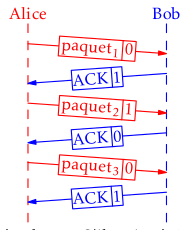
\includegraphics{images/bit_alterne1.png}\\

\emph{Déroulement du protocole du bit alterné}

\begin{itemize}
\item
  Le système de bit de contrôle est complété avec un système d'horloge
  côté émetteur. Un ``chronomètre'' est déclenché à chaque envoi de
  paquet. Si au bout d'un certain temps (le \emph{timeout}), l'émetteur
  n'a pas reçu un \emph{accusé de réception} correct (avec le bon bit de
  contrôle), la trame précédemment envoyée par l'émetteur est considérée
  comme perdue et elle est de nouveau envoyée.
\item
  Considérons quelques cas de perte de paquet :

  \begin{itemize}
  \tightlist
  \item
    Si un paquet (avec par exemple le bit de contrôle0) envoyé par
    l'émetteur est perdu, l'accusé de réception ne lui revient pas au
    bout du timeout, il comprend que son paquet a été perdu et il
    renvoie le paquet.
  \item
    Si l'\emph{accusé de réception} avec le bit de contrôle 1 est perdu,
    il ne parvient pas à l'émetteur au bout du \emph{timeout} qui
    renvoie le paquet avec le bit de contrôle 0. Le destinataire reçoit
    un paquet avec le bit de contrôle 0 alors qu'il attendait le bit de
    contrôle 1. Il comprend que son acquittement a été perdu et il
    renvoie son acquittement avec le bit de contrôle 1.
  \end{itemize}
\end{itemize}

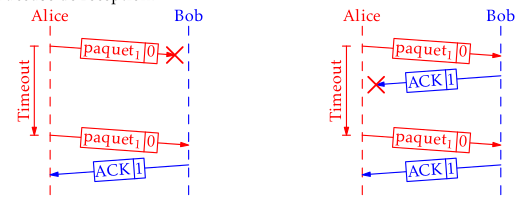
\includegraphics{images/bit_alterne2.png}\\

\emph{Pertes de paquets dans le protocole du bit alterné}

\end{cours}

\hypertarget{applications}{%
\subsection{Applications}\label{applications}}

\begin{exercice}{}

\begin{enumerate}
\def\labelenumi{\arabic{enumi}.}
\item
  Dans quel but le protocole du bit alterné peut-il être utilisé ?

  \begin{itemize}
  \tightlist
  \item
    \textbf{Réponse A :} Pour chiffrer des données lors de transmission
    de données sur un réseau
  \item
    \textbf{Réponse B :} Pour détecter des pertes de paquets de données
    lors de transmission de données sur un réseau.
  \item
    \textbf{Réponse C :} Pour créer des paquets de données lors de
    transmission de données sur un réseau.
  \item
    \textbf{Réponse D :} Pour envoyer les paquets de données à la bonne
    l'adresse IP de la machine de destination.
  \end{itemize}
\item
  Quelle est la réponse à envoyer quand on reçoit un paquet avec le bit
  de contrôle 1 ?
\item
  On arrive au timeout pour le paquet n avec un bit de contrôle de 0.
  Quelle était la réponse attendue ?
\item
  Imaginer une ou plusieurs situations où le protocole de bit alterné
  est inefficace et ne permet pas de récupérer un paquet perdu.
\end{enumerate}

\end{exercice}

\end{document}
